\documentclass[11pt,a4paper]{article}
\usepackage{float}
\usepackage{amsmath, amssymb, amsthm}
\usepackage{geometry}
\usepackage{graphicx}
\usepackage{url}
\usepackage{hyperref}
\usepackage[dvipsnames]{xcolor}
\usepackage{mylistings}
\usepackage[font=small,skip=4pt]{caption}
\usepackage{chngcntr,tocloft}

\counterwithin*{figure}{section}
\counterwithin*{figure}{subsection}
\counterwithin*{figure}{subsubsection}

\addtolength{\cftfignumwidth}{2em}


\renewcommand{\thefigure}{%
  \ifnum\value{subsection}=0
    \thesection.\arabic{figure}%
  \else
    \ifnum\value{subsubsection}=0
      \thesubsection.\arabic{figure}%
    \else
      \thesubsubsection.\arabic{figure}%
    \fi
  \fi
}

\renewcommand{\lstlistingname}{Code}

\definecolor{codegreen}{rgb}{0,0.6,0}
\definecolor{codegray}{rgb}{0.5,0.5,0.5}
\definecolor{codepurple}{rgb}{0.58,0,0.82}
\definecolor{backcolour}{rgb}{0.9725,0.9725,0.9725}

\lstdefinestyle{mystyle}{
backgroundcolor=\color{backcolour},   
commentstyle=\color{codegreen},
keywordstyle=\color{magenta},
% numberstyle=\tiny\color{codegray},
stringstyle=\color{codepurple},
basicstyle=\ttfamily\footnotesize,
breakatwhitespace=false,         
breaklines=true,                 
captionpos=t,                    
keepspaces=true,                 
% numbers=left,                    
% numbersep=5pt,                  
showspaces=false,                
showstringspaces=false,
showtabs=false,                  
tabsize=2,
frame=tb,
framexleftmargin=2mm,
xleftmargin=2mm,
framexrightmargin=2mm,
xrightmargin=2mm,
% rulecolor=\color{black},
upquote=true,
aboveskip=3mm,
belowskip=3mm
}

\lstset{style=mystyle}

\parindent 0pt

\geometry{left=0.75in, right=0.75in, top=1in, bottom=1in}
\renewcommand{\contentsname}{Contents}

\renewcommand{\baselinestretch}{1.25}
\renewcommand{\contentsname}{Contents}

\usepackage{hyperref}
\hypersetup{
    colorlinks,
    citecolor=blue,
    filecolor=blue,
    linkcolor=blue,
    urlcolor=blue
}

\usepackage{enumitem}

\usepackage{cleveref}
\crefname{section}{\S}{\S\S}
\Crefname{section}{\S}{\S\S}
\crefname{subsection}{\S}{\S\S}
\Crefname{subsection}{\S}{\S\S}

\begin{document}

% Titlepage
\newpage
\begin{titlepage}
  \vspace*{\fill} % add vertical space before content
  \centering
  \huge{\textbf{CS477 -- Computer Vision}} \\
  \huge{Fall 2023} \\
  \huge{Assignment 2} \\ [0.75cm]
  \begin{figure}[ht!]
    \centering
    
\includegraphics[width=0.5\textwidth]{figs/nust.pdf}
  \end{figure}
  \vspace {0.75cm}
  \Large{By} \\
  \Large{\textbf{Muhammad Umer}\quad(CMS -- 345834)} \\ [0.75cm]
  \Large{Instructor} \\
  \Large{\textbf{Dr. Mohsin Kamal}} \\[0.75cm]
  \Large{School of Electrical Engineering and Computer Science (SEECS) \\
    National University of Sciences and Technology (NUST) \\
    Islamabad, Pakistan} \\ [0.75cm]
  \Large{\today}
  \vspace*{\fill} % add vertical space after content
\end{titlepage}

\tableofcontents

\newpage
\setcounter{page}{1}
\section{Introduction}

In this assignment, we delve into the world of feature detection and matching. We will be implementing the SIFT algorithm from scratch and use it to find correspondences between keypoints in a pair of images. We will also be exploring the methods of image stitching and stitch any two images.

\subsection*{Deliverables}
\begin{enumerate}[leftmargin=*]
  \item \textbf{SIFT Algorithm:}
        \textit{\\Implement the SIFT algorithm from scratch in Python/MATLAB. Apply your implementation to a pair of images and find correspondences between keypoints.}

  \item \textbf{Image Stitching:}
        \textit{\\Discover the methods of image stitching and stitch any two images.}
\end{enumerate}

\subsection*{Notes}
\begin{enumerate}[label=(\alph*), leftmargin=*]
  \item Submit the solution of the assignment in soft form and MATLAB/python files on LMS.
  \item You are encouraged to use standard image processing libraries (e.g., OpenCV) for low-level operations (e.g., image loading, convolution). However, the core algorithms should be implemented from scratch.
  \item Avoid using pre-built functions for the core components of the algorithms.
  \item Provide comparisons between your implementations and the results obtained using established libraries/functions where applicable.
  \item Ensure your code is well-commented and organized.
\end{enumerate}

\subsection*{Copying}
Copying is highly discouraged and it will lead to a significant loss  (90-95 \%) of marks.

\textit{*Copying includes using sentences, variables, code, formats from others. Discussion is appreciated, but attempt the tasks on your own (which would make it look original).}

\newpage
\section{Task 1 -- SIFT Algorithm}

We implement the SIFT algorithm from scratch, but only to a reasonable extent. The author of this report has implemented core components of the algorithm from scratch, but has used pre-defined functions for operations such as hessian matrix computation, extremum interpolation, and orientation assignment.

We begin by importing the required libraries.
% Importing libraries
\begin{lstlisting}[language=Python, caption=Importing libraries]
  import math
  from copy import deepcopy
  from functools import cmp_to_key
  
  import cv2
  import matplotlib.pyplot as plt
  
  from sift_utils import (
      extrema_interpolated_fit,
      get_histogram_bins,
      get_keypoint_orientations,
      process_bins,
  )
  
  plt.rcParams["font.family"] = "STIXGeneral"
  import numpy as np
\end{lstlisting}

From hereon, assume that all of the code-listings are in the function \lstinline[columns=fixed]{task1(img_path, save=False)}. We initialize the parameters for SIFT, and load the images.

\begin{lstlisting}[language=Python, caption=Initializing parameters and loading images]
  img = cv2.imread(img_path)
  img = cv2.cvtColor(img, cv2.COLOR_BGR2RGB)
  rgb_img = deepcopy(img)

  plt.imshow(img)
  plt.title("Original Image")
  plt.tight_layout()
  if save:
      plt.savefig(
          "report/figs/original.png", dpi=300, bbox_inches="tight", pad_inches=0
      )

  img = cv2.cvtColor(img, cv2.COLOR_RGB2GRAY)
  gray_img = deepcopy(img)
  img = cv2.resize(img, (0, 0), fx=2, fy=2)  # upsample image for better results
  img = img.astype(float)

  sigma_i = 1.44  # initial sigma
  sigma = sigma_i
  # match size of kernel from opencv
  size = 2 * math.ceil(3 * sigma) + 1
  cv_img = cv2.GaussianBlur(img, (0, 0), sigma)
  kernel = gaussian_kernel(size, sigma)
  img = cv2.filter2D(img, -1, kernel)
  plt.imshow(img, cmap="gray")
  plt.title("Upsampled & Blurred")
  plt.tight_layout()
  if save:
      plt.savefig(
          "report/figs/upsampled_blurred.png",
          dpi=300,
          bbox_inches="tight",
          pad_inches=0,
      )
  plt.show()
\end{lstlisting}

% 2 subfigures, each with different caption
\begin{figure}[ht!]
  \centering
  \begin{minipage}{0.45\textwidth}
    \centering
    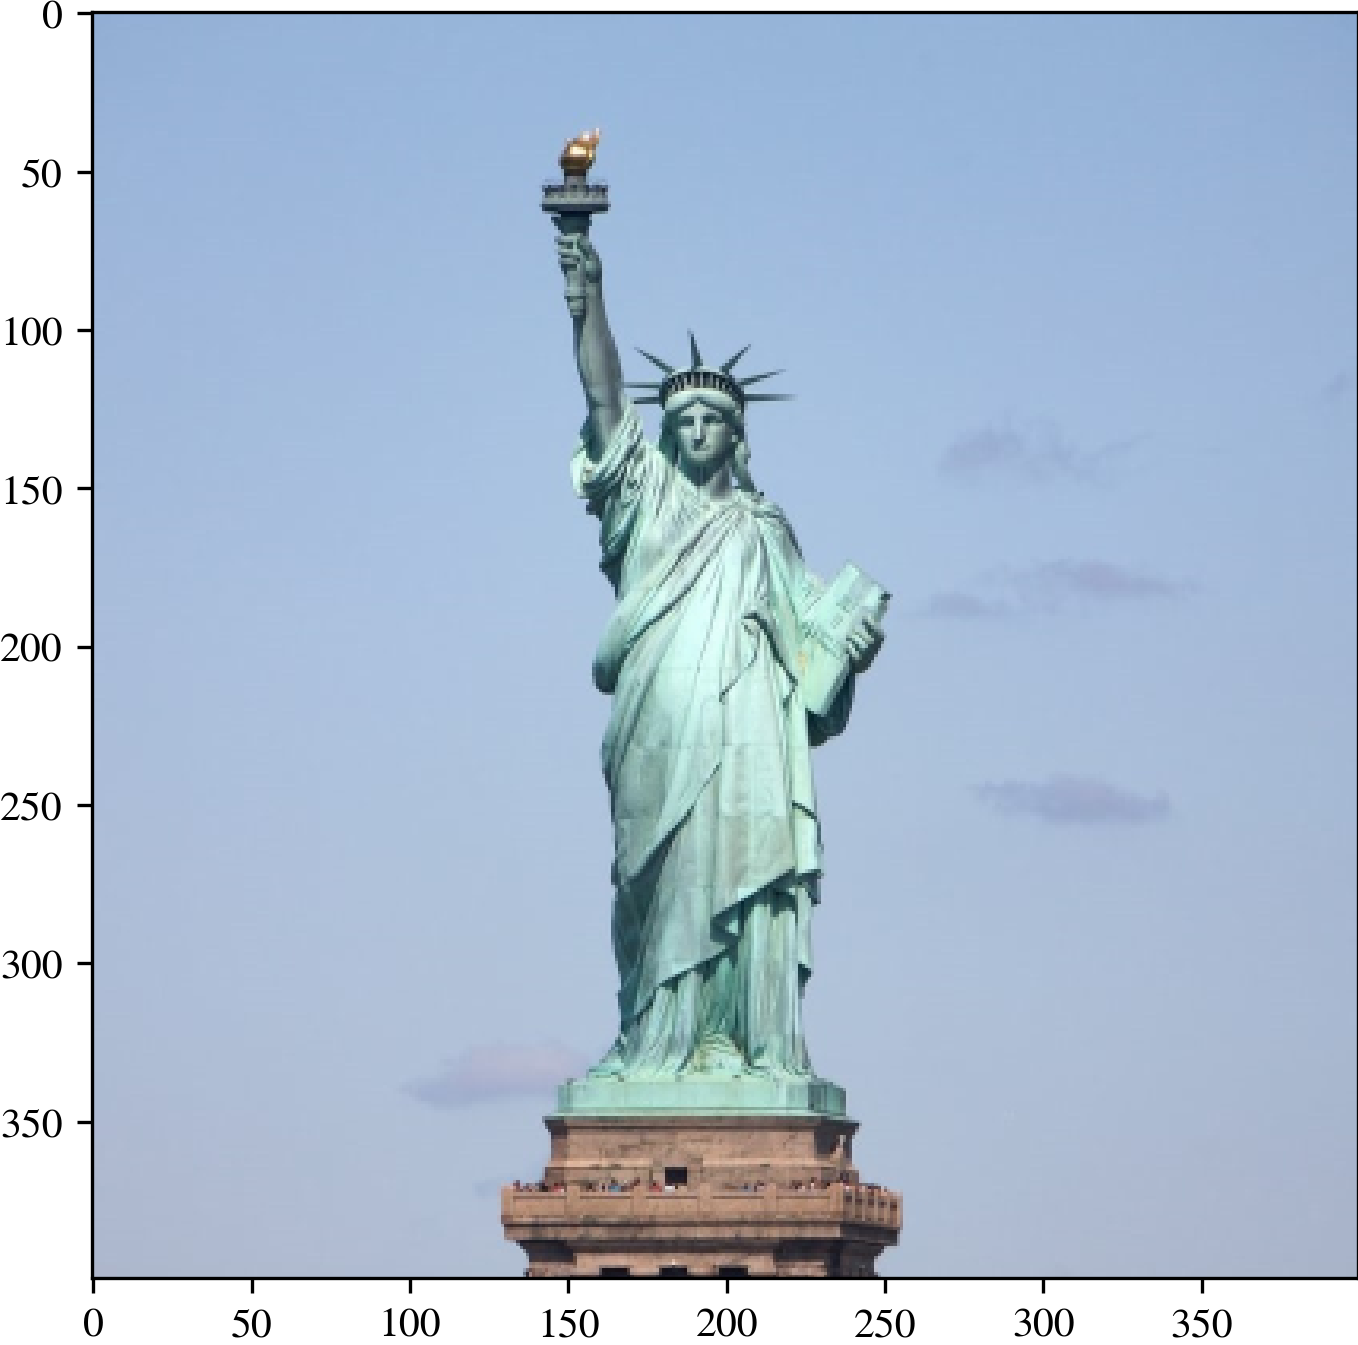
\includegraphics[width=0.9\textwidth]{figs/original.png} % first figure itself
    \caption{Original Image}
  \end{minipage}
  \quad
  \begin{minipage}{0.45\textwidth}
    \centering
    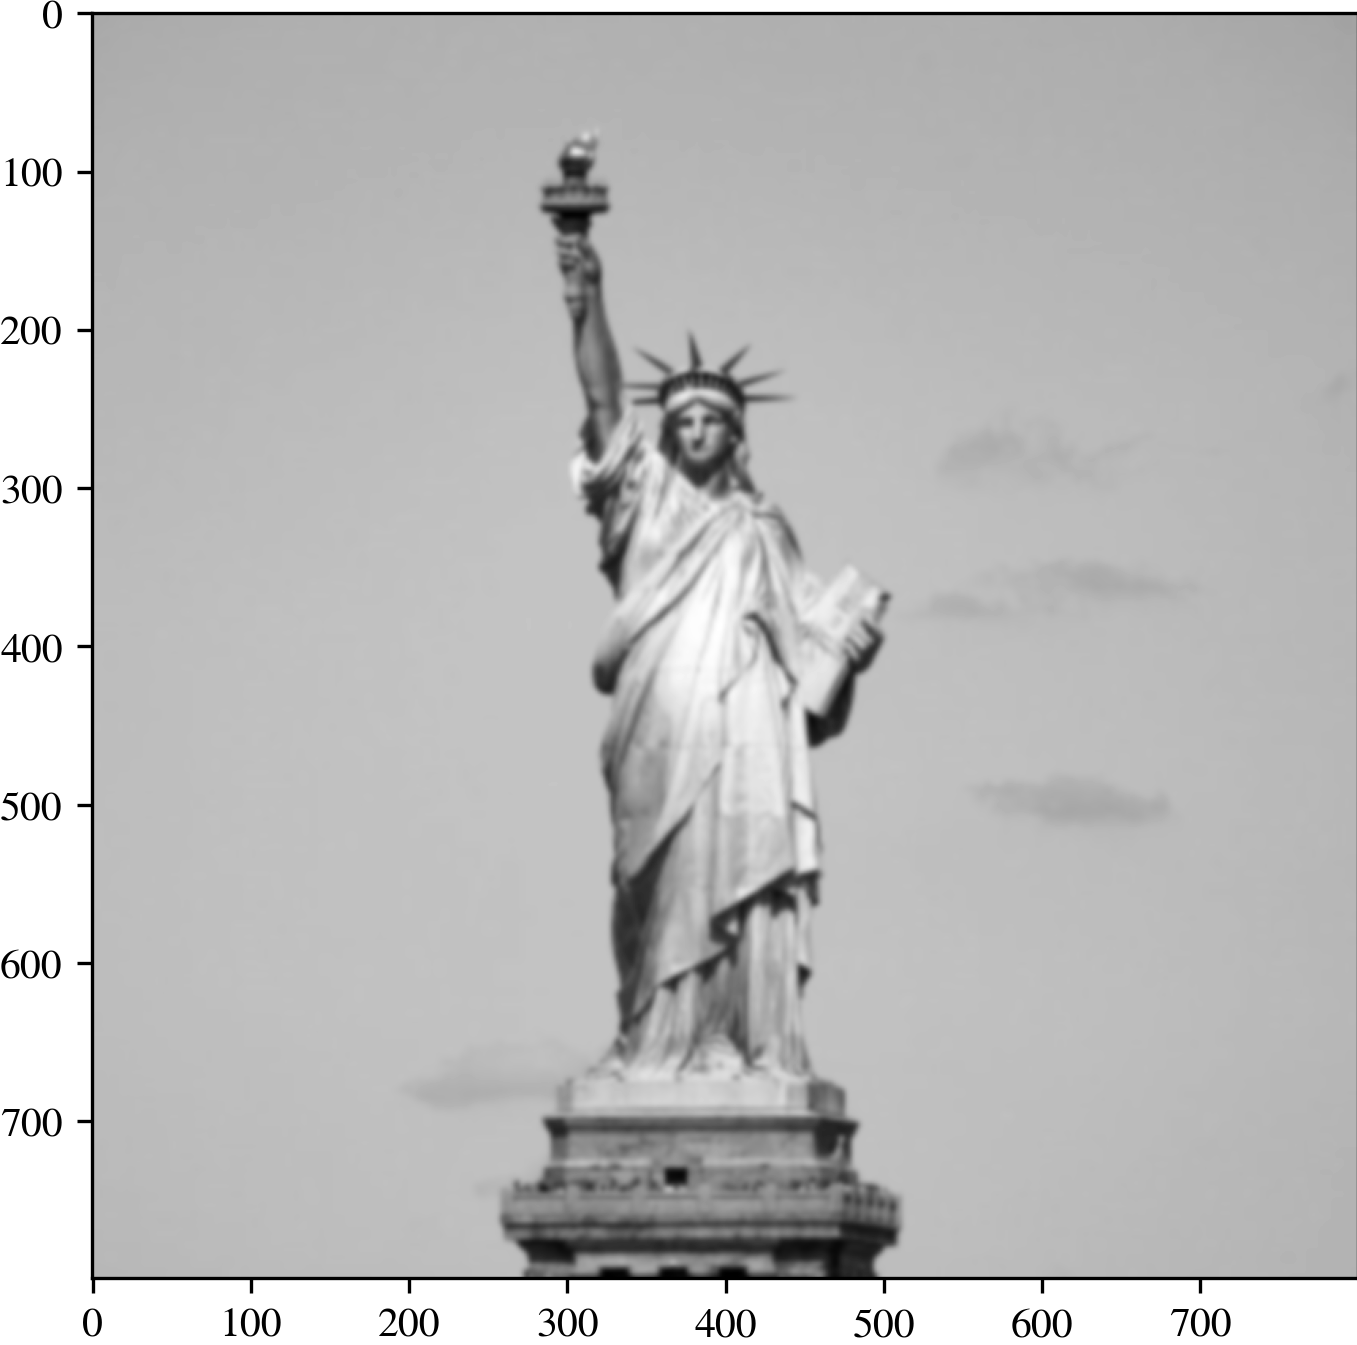
\includegraphics[width=0.9\textwidth]{figs/upsampled_blurred.png} % second figure itself
    \caption{Upsampled \& Blurred}
  \end{minipage}
\end{figure}

The SIFT algorithm comprises of four steps:

\begin{enumerate}[leftmargin=*]
  \item Scale-space peak detection
  \item Keypoint localization
  \item Orientation assignment
  \item Keypoint descriptor
\end{enumerate}

The code-listings for each of these steps are provided below.

\begin{lstlisting}[language=Python, caption=Scale-space peak detection]
  N_o = 4  # number of octaves
  N_i = 3  # number of intervals

  k = 2 ** (1 / N_i)  # scale factor
  sigma_list = [sigma]

  # Number of images in each octave = N_i + 3
  # +3 as we require 2 extra images for DoG and 1 extra image for Gaussian blur
  for i in range(1, N_i + 3):
      sigma = (k ** (i - 1)) * sigma
      sigma_cum = k * sigma
      sigma_list.append(np.sqrt(sigma_cum**2 - sigma**2))

  # Generate octave images
  ss_img = deepcopy(img)
  octave_images = []
  for i in range(N_o):
      # Generate Gaussian images
      gaussian_images = []
      for j in sigma_list:
          # the first image is just the base image
          if j == sigma_list[0]:
              gaussian_images.append(ss_img)
              continue
          size = 2 * math.ceil(3 * j) + 1  # match size of kernel from opencv
          kernel = gaussian_kernel(size, j)  # generate gaussian kernel
          blur_img = cv2.filter2D(ss_img, -1, kernel)
          gaussian_images.append(blur_img)
      octave_images.append(gaussian_images)
      base_img = gaussian_images[
          -3
      ]
      ss_img = cv2.resize(
          base_img, (0, 0), fx=0.5, fy=0.5
      )  # downsample image for next octave

  # Generate DoG images
  dog_images = []
  for i in range(N_o):
      difference = []
      for j in zip(octave_images[i], octave_images[i][1:]):
          difference.append(j[1] - j[0])
      dog_images.append(difference)

  # Visualize Scale-space pyramid octave 1
  nr_cols = len(octave_images)
  nr_rows = len(octave_images[0])
  fig, axs = plt.subplots(
      nr_rows,
      nr_cols,
      figsize=(6, 10),
      gridspec_kw={"wspace": 0, "hspace": 0},
      squeeze=True,
  )

  for col, octave in enumerate(octave_images):
      for row, layer in enumerate(octave):
          axs[row][col].axis("off")
          axs[row][col].imshow(layer, cmap="gray", aspect="auto")

  fig.suptitle("Gaussian Octaves")
  fig.supxlabel("Octave Index")
  fig.supylabel("Blur Level")
  plt.tight_layout()
  if save:
      plt.savefig(
          "report/figs/gaussian_octaves.png",
          dpi=300,
          bbox_inches="tight",
          pad_inches=0,
      )

  # Visualize Scale-space pyramid octave 1
  nr_cols = len(dog_images)
  nr_rows = len(dog_images[0])
  fig, axs = plt.subplots(
      nr_rows,
      nr_cols,
      figsize=(6, 10),
      gridspec_kw={"wspace": 0, "hspace": 0},
      squeeze=True,
  )

  for col, octave in enumerate(dog_images):
      for row, layer in enumerate(octave):
          axs[row][col].axis("off")
          axs[row][col].imshow(layer, cmap="gray", aspect="auto")

  fig.suptitle("DoG Octaves")
  fig.supxlabel("Octave Index")
  fig.supylabel("Blur Level")
  plt.tight_layout()
  if save:
      plt.savefig(
          "report/figs/dog_octaves.png",
          dpi=300, bbox_inches="tight", pad_inches=0
      )
\end{lstlisting}

% 2 subfigures, each with different caption
\begin{figure}[ht!]
  \centering
  \begin{minipage}{0.45\textwidth}
    \centering
    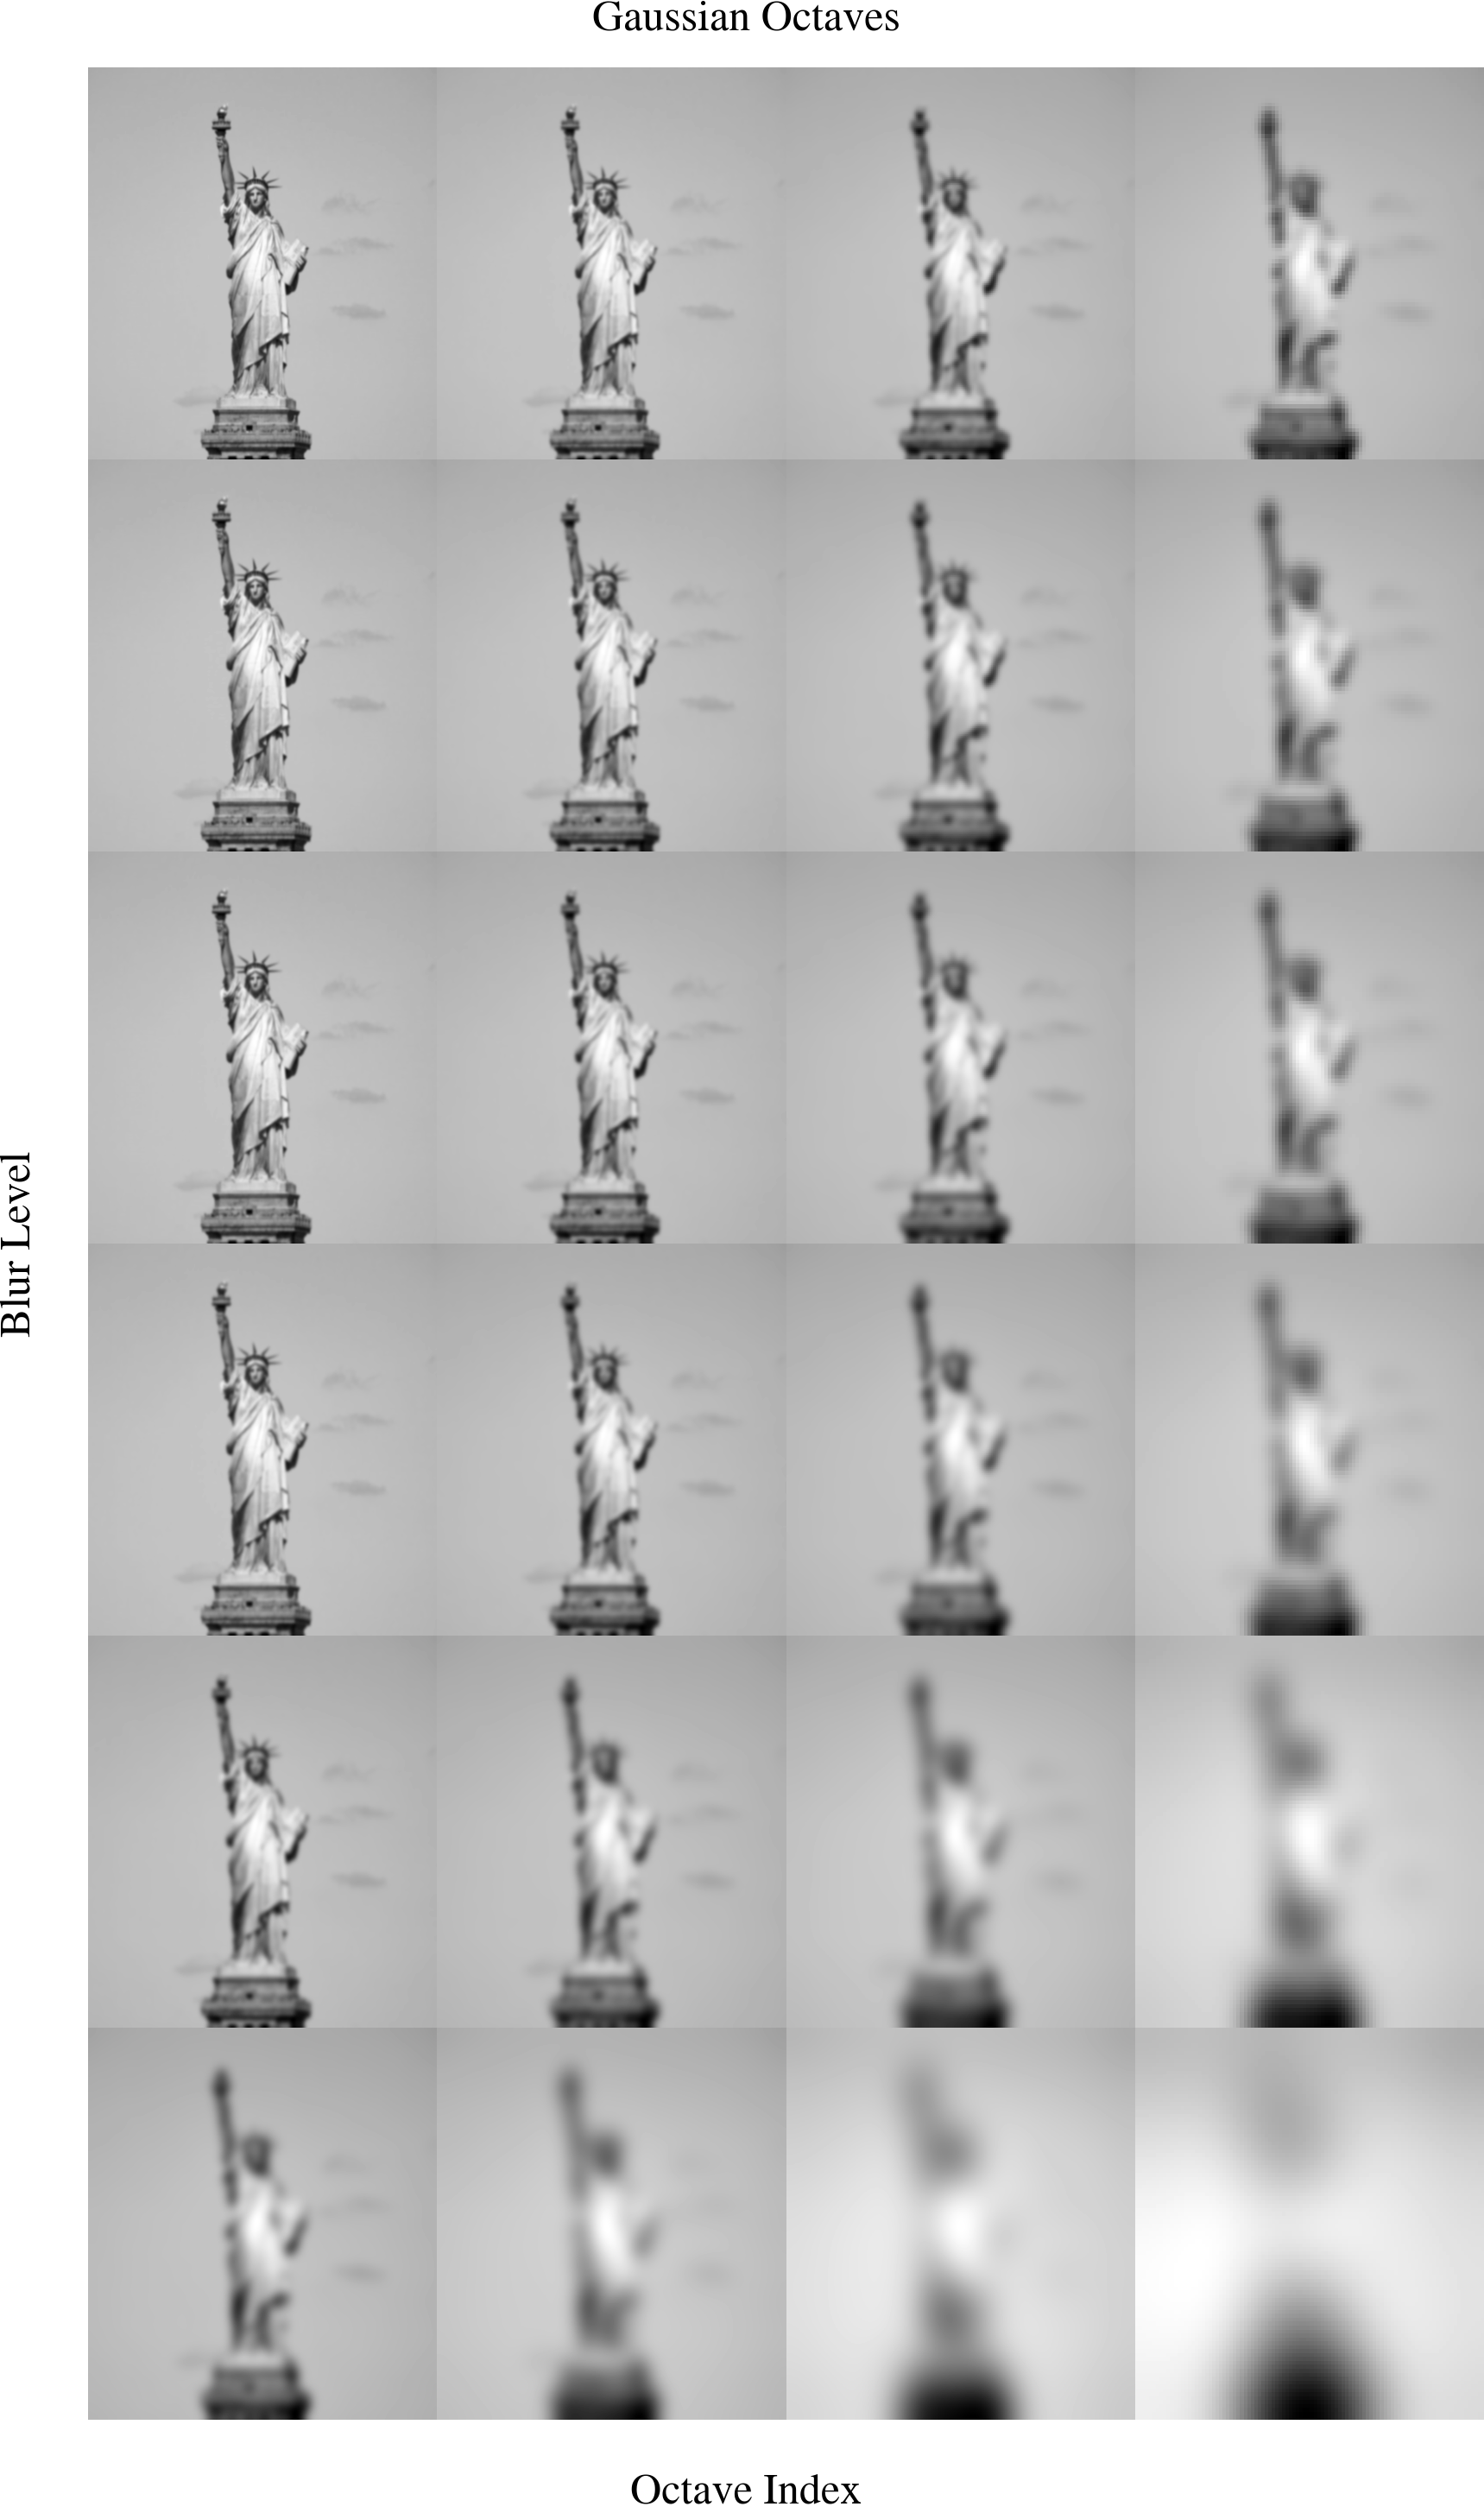
\includegraphics[width=0.9\textwidth]{figs/gaussian_octaves.png} % first figure itself
    \caption{Gaussian Octaves}
  \end{minipage}
  \quad
  \begin{minipage}{0.45\textwidth}
    \centering
    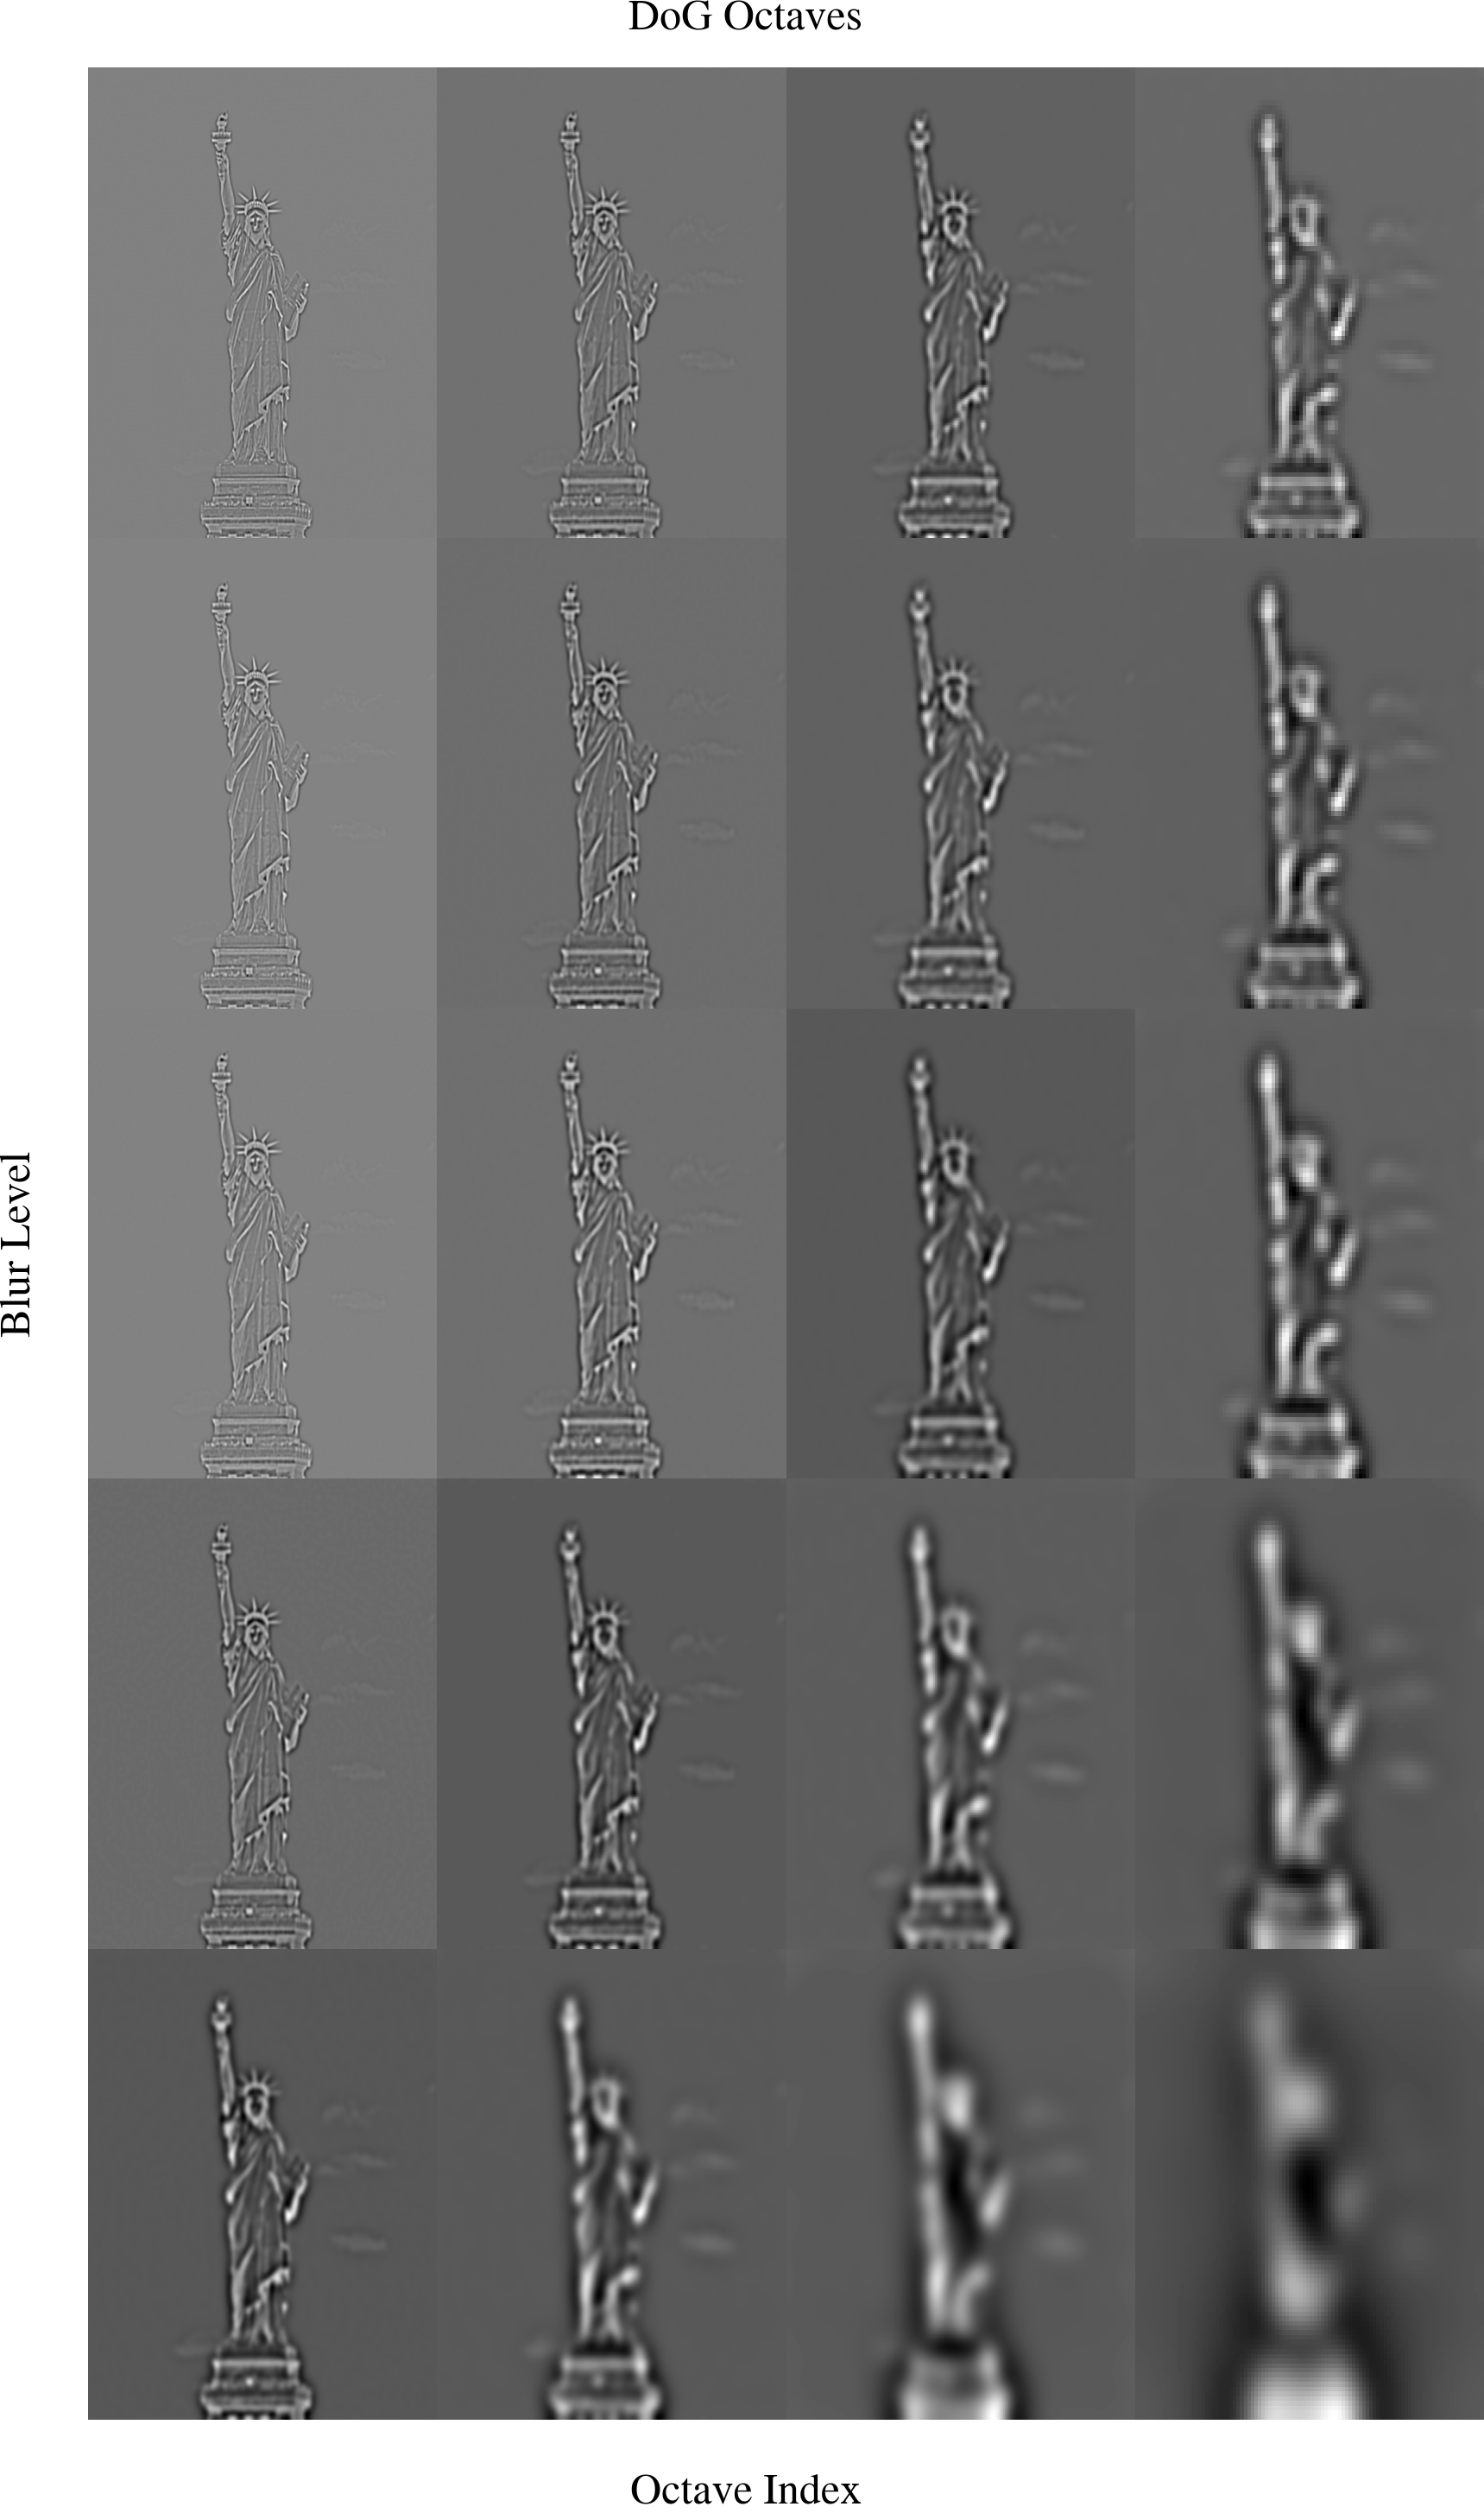
\includegraphics[width=0.9\textwidth]{figs/dog_octaves.png} % second figure itself
    \caption{DoG Octaves}
  \end{minipage}
\end{figure}

\newpage

\begin{lstlisting}[language=Python, caption=Keypoint localization]
  low_contrast_thresh = 0.04
  r = 5  # radius of the area considered for comparison with neighbors

  threshold = np.floor(
      0.5 * low_contrast_thresh / N_i * 255
  )  # from OpenCV implementation

  localized_keypoints = []
  octave_indices = []
  localization_indices = []

  def check_extrema(low, center, high, threshold):
      center_pixel_value = center[1, 1]

      # Check if the center pixel is an extrema
      if abs(center_pixel_value) > threshold:
          is_positive = center_pixel_value > 0
          is_negative = center_pixel_value < 0

          if is_positive:
              return (
                  np.all(center_pixel_value >= low)
                  and np.all(center_pixel_value >= high)
                  and np.all(center_pixel_value >= center[0, :])
                  and np.all(center_pixel_value >= center[2, :])
                  and center_pixel_value >= center[1, 0]
                  and center_pixel_value >= center[1, 2]
              )
          elif is_negative:
              return (
                  np.all(center_pixel_value <= low)
                  and np.all(center_pixel_value <= high)
                  and np.all(center_pixel_value <= center[0, :])
                  and np.all(center_pixel_value <= center[2, :])
                  and center_pixel_value <= center[1, 0]
                  and center_pixel_value <= center[1, 2]
              )
      return False

  for octave_idx, dog_oct in enumerate(dog_images):
      for img_idx, (img1, img2, img3) in enumerate(
          zip(dog_oct, dog_oct[1:], dog_oct[2:])
      ):
          # Loop over all the pixels in the image
          for x in range(r, img1.shape[0] - r):
              for y in range(r, img1.shape[1] - r):
                  # Check if the current pixel is an extrema
                  if check_extrema(
                      img1[x - 1 : x + 2, y - 1 : y + 2],
                      img2[x - 1 : x + 2, y - 1 : y + 2],
                      img3[x - 1 : x + 2, y - 1 : y + 2],
                      threshold,
                  ):
                      # If pixel is an extrema, perform an interpolated fit
                      loc_res = extrema_interpolated_fit(
                          x, y, img_idx + 1, octave_idx, N_i,
                          dog_oct, sigma_i, low_contrast_thresh, r)
                      # Add the keypoints to the list
                      if loc_res is not None:
                          keypoint, idx = loc_res
                          localized_keypoints.append(keypoint)
                          octave_indices.append(octave_idx)
                          localization_indices.append(idx)

  fig, ax = plt.subplots()
  ax.imshow(img, cmap="gray")
  for keypoint in localized_keypoints:
      ax.scatter(keypoint.pt[0], keypoint.pt[1], s=1, c="r")
  plt.tight_layout()
  if save:
      plt.savefig("report/figs/keypoints.png",
                   dpi=300, bbox_inches="tight", pad_inches=0)
\end{lstlisting}

\begin{figure}[ht!]
  \centering
  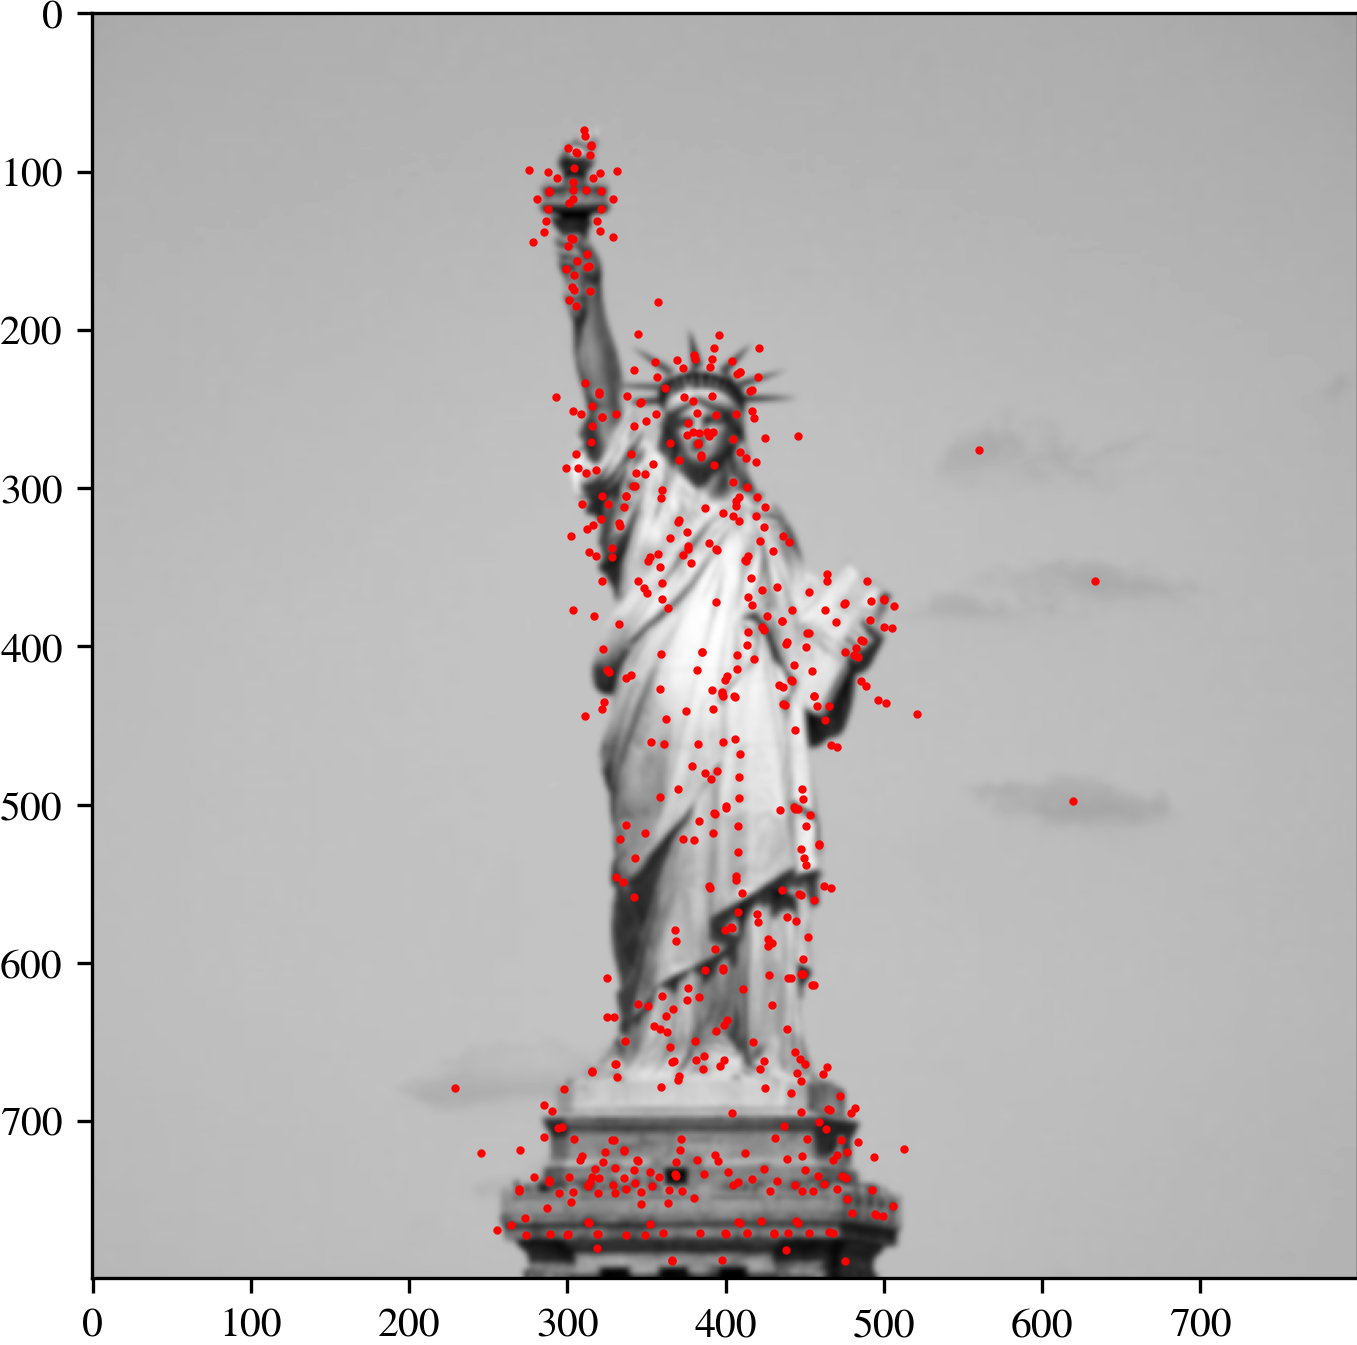
\includegraphics[width=0.5\textwidth]{figs/keypoints.png}
  \caption{Localized Keypoints}
\end{figure}

\begin{lstlisting}[language=Python, caption=Orientation assignment]
  orientations = []
  for keypoint, octave_idx, localization_idx in zip(
      localized_keypoints, octave_indices, localization_indices
  ):
      ort_keypoints = get_keypoint_orientations(
          keypoint, octave_idx, octave_images[octave_idx][idx])
      orientations.extend(ort_keypoints)

  def compare_keypoints(keypoint1, keypoint2):
      if keypoint1.pt[0] != keypoint2.pt[0]:
          return keypoint1.pt[0] - keypoint2.pt[0]
      if keypoint1.pt[1] != keypoint2.pt[1]:
          return keypoint1.pt[1] - keypoint2.pt[1]
      if keypoint1.size != keypoint2.size:
          return keypoint2.size - keypoint1.size
      if keypoint1.angle != keypoint2.angle:
          return keypoint1.angle - keypoint2.angle
      if keypoint1.response != keypoint2.response:
          return keypoint2.response - keypoint1.response
      if keypoint1.octave != keypoint2.octave:
          return keypoint2.octave - keypoint1.octave
      return keypoint2.class_id - keypoint1.class_id

  orientations.sort(key=cmp_to_key(compare_keypoints))
  unique_keypoints = [orientations[0]]

  # Remove duplicate keypoints
  for ort_keypoint in orientations[1:]:
      if (
          unique_keypoints[-1].pt[0] == ort_keypoint.pt[0]
          and unique_keypoints[-1].pt[1] == ort_keypoint.pt[1]
          and unique_keypoints[-1].size == ort_keypoint.size
          and unique_keypoints[-1].angle == ort_keypoint.angle
      ):
          continue
      unique_keypoints.append(ort_keypoint)

  # convert keypoints to original scale
  converted_keypoints = []

  for keypoint in unique_keypoints:
      keypoint.pt = (keypoint.pt[0] * 0.5, keypoint.pt[1] * 0.5)
      keypoint.size *= 0.5
      keypoint.octave = (keypoint.octave & ~255) | \
                        ((keypoint.octave - 1) & 255)
      converted_keypoints.append(keypoint)

  # Visualize keypoints
  fig, ax = plt.subplots()
  ax.imshow(rgb_img, cmap="gray")

  for keypoint in converted_keypoints:
      ax.scatter(keypoint.pt[0], keypoint.pt[1], s=1, c="r")
      
  plt.tight_layout()
  if save:
      plt.savefig(
          "report/figs/scaled_keypoints.png",
          dpi=300, bbox_inches="tight", pad_inches=0)
\end{lstlisting}

\begin{figure}[ht!]
  \centering
  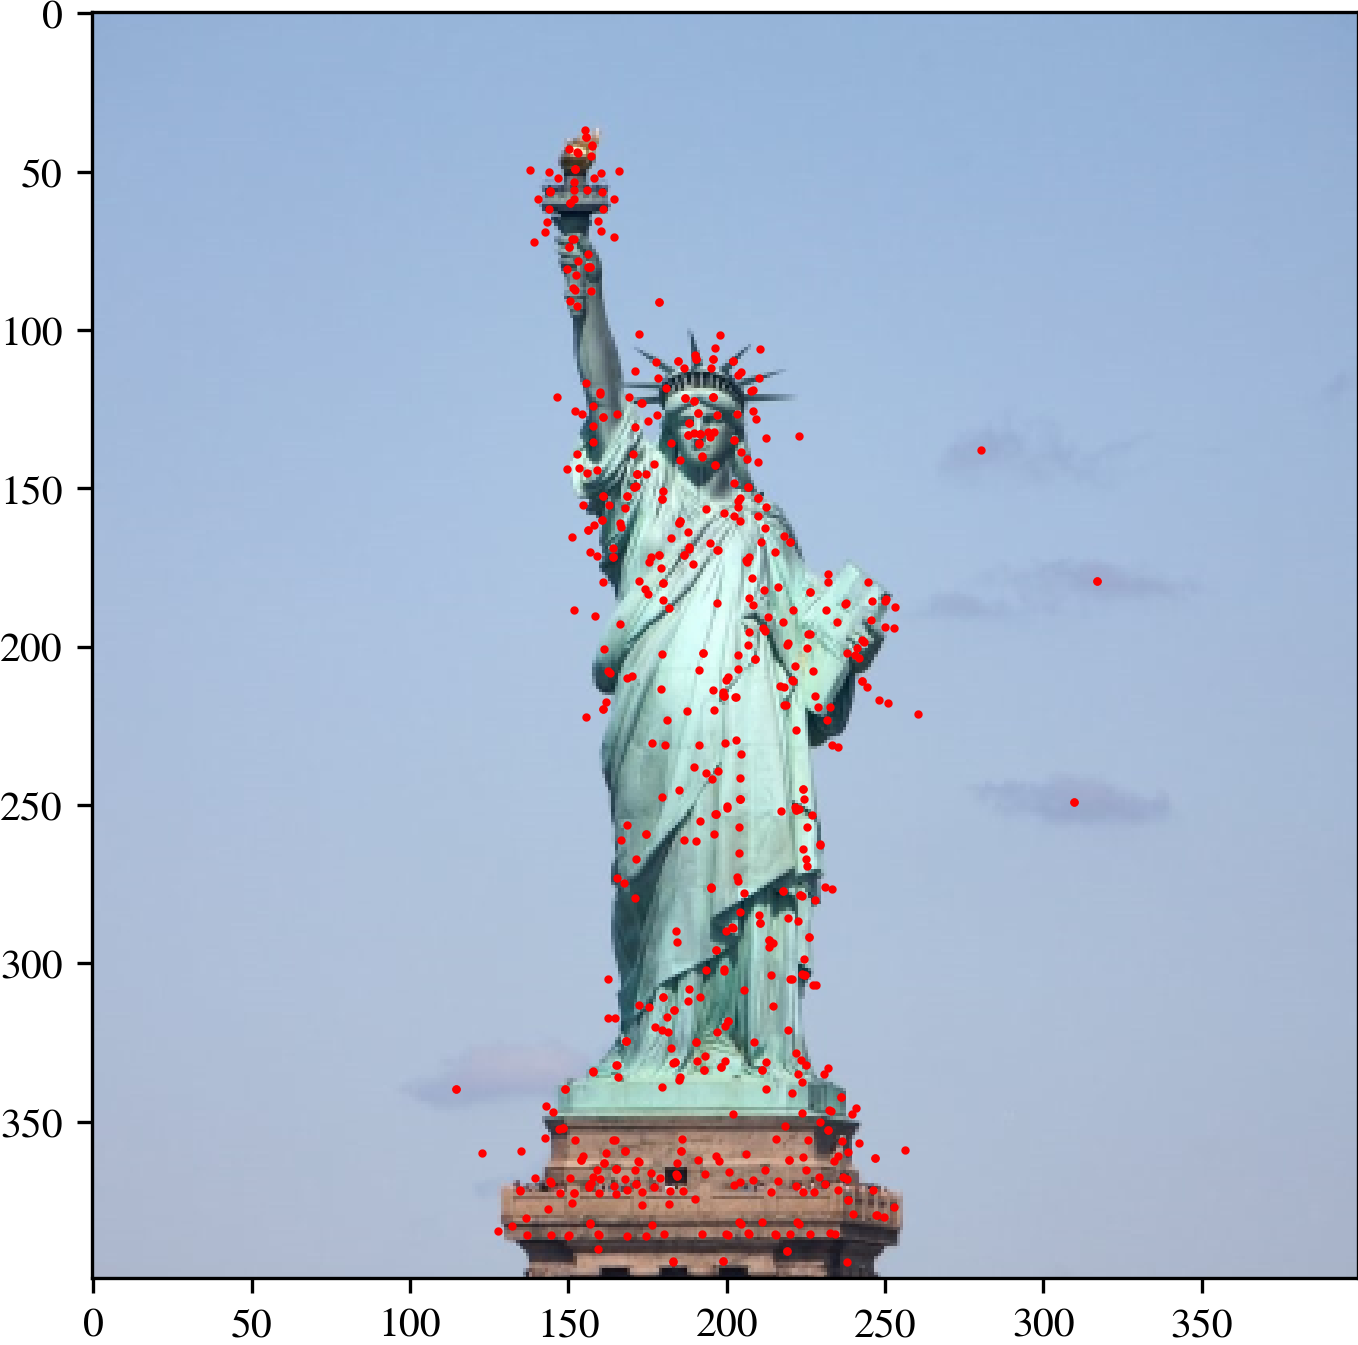
\includegraphics[width=0.5\textwidth]{figs/scaled_keypoints.png}
  \caption{Keypoints $\rightarrow$ Original Scale}
\end{figure}

\newpage

\begin{lstlisting}[language=Python, caption=Keypoint descriptor]
  descriptors = []
  window_width = 4  # Size of the window for the descriptor
  num_bins = 8  # Number of bins for the histogram
  scale_multiplier = 3
  descriptor_max_value = 0.2

  for keypoint in converted_keypoints:
      octave = keypoint.octave & 255  # Extract octave from keypoint
      layer = (keypoint.octave >> 8) & 255  # Extract layer from keypoint

      # Handle negative octave values
      octave = octave | -128 if octave >= 128 else octave

      # Calculate scale based on octave
      scale = 1 / np.float32(2**octave) if octave >= 0 else np.float32(2**-octave)
      octave_images = np.array(octave_images, dtype=object)
      gaussian_image = octave_images[
          octave + 1, layer
      ]  # Get the Gaussian image for the octave and layer
      num_rows, num_cols = gaussian_image.shape
      point = np.round(scale * np.array(keypoint.pt)).astype(
          "int"
      )  # Scale the keypoint
      bins_per_degree = num_bins / 360.0  # Calculate bins per degree
      angle = 360.0 - keypoint.angle  # Calculate angle
      cos_angle = np.cos(np.deg2rad(angle))  # Calculate cosine of angle
      sin_angle = np.sin(np.deg2rad(angle))  # Calculate sine of angle
      weight_multiplier = -0.5 / (
          (0.5 * window_width) ** 2
      )  # Calculate weight multiplier
      row_bins = []
      col_bins = []
      magnitudes = []
      orientation_bins = []
      histogram_tensor = np.zeros(
          (window_width + 2, window_width + 2, num_bins)
      )  # Initialize histogram tensor

      # Calculate descriptor window size
      hist_width = scale_multiplier * 0.5 * scale * keypoint.size
      half_width = int(round(hist_width * np.sqrt(2) * (window_width + 1) * 0.5))
      half_width = int(min(half_width, np.sqrt(num_rows**2 + num_cols**2)))

      # Populate histogram_tensor
      row_bins, col_bins, magnitudes, orientation_bins = get_histogram_bins(
          point,
          gaussian_image,
          angle,
          hist_width,
          window_width,
          weight_multiplier,
          bins_per_degree,
      )

      process_bins(
          row_bins, col_bins, magnitudes, orientation_bins, num_bins, histogram_tensor
      )
      descriptor_vector = histogram_tensor[
          1:-1, 1:-1, :
      ].flatten()  # Remove histogram borders

      # Threshold and normalize descriptor_vector
      threshold = np.linalg.norm(descriptor_vector) * descriptor_max_value
      descriptor_vector[descriptor_vector > threshold] = threshold
      descriptor_vector /= max(np.linalg.norm(descriptor_vector), 1e-7)
      descriptor_vector = np.round(512 * descriptor_vector)
      descriptor_vector[descriptor_vector < 0] = 0
      descriptor_vector[descriptor_vector > 255] = 255
      descriptors.append(descriptor_vector)  # Add descriptor to list

  image_with_keypoints = deepcopy(rgb_img)  # Create a copy of the image to draw on

  for keypoint, descriptor in zip(converted_keypoints, descriptors):
      # Extract keypoint information
      x, y = map(int, keypoint.pt)
      size = int(keypoint.size)
      angle = keypoint.angle

      # Draw the keypoint
      cv2.circle(image_with_keypoints, (x, y), size, (0, 255, 0), 1)
      cv2.line(
          image_with_keypoints,
          (x, y),
          (
              int(x + size * np.cos(np.radians(angle))),
              int(y + size * np.sin(np.radians(angle))),
          ),
          (0, 0, 0),
          1,
      )

  plt.imshow(image_with_keypoints)
  plt.tight_layout()
  if save:
      plt.savefig(
          "report/figs/keypoints_with_descriptors.png",
          dpi=300, bbox_inches="tight", pad_inches=0)
\end{lstlisting}

\begin{figure}[ht!]
  \centering
  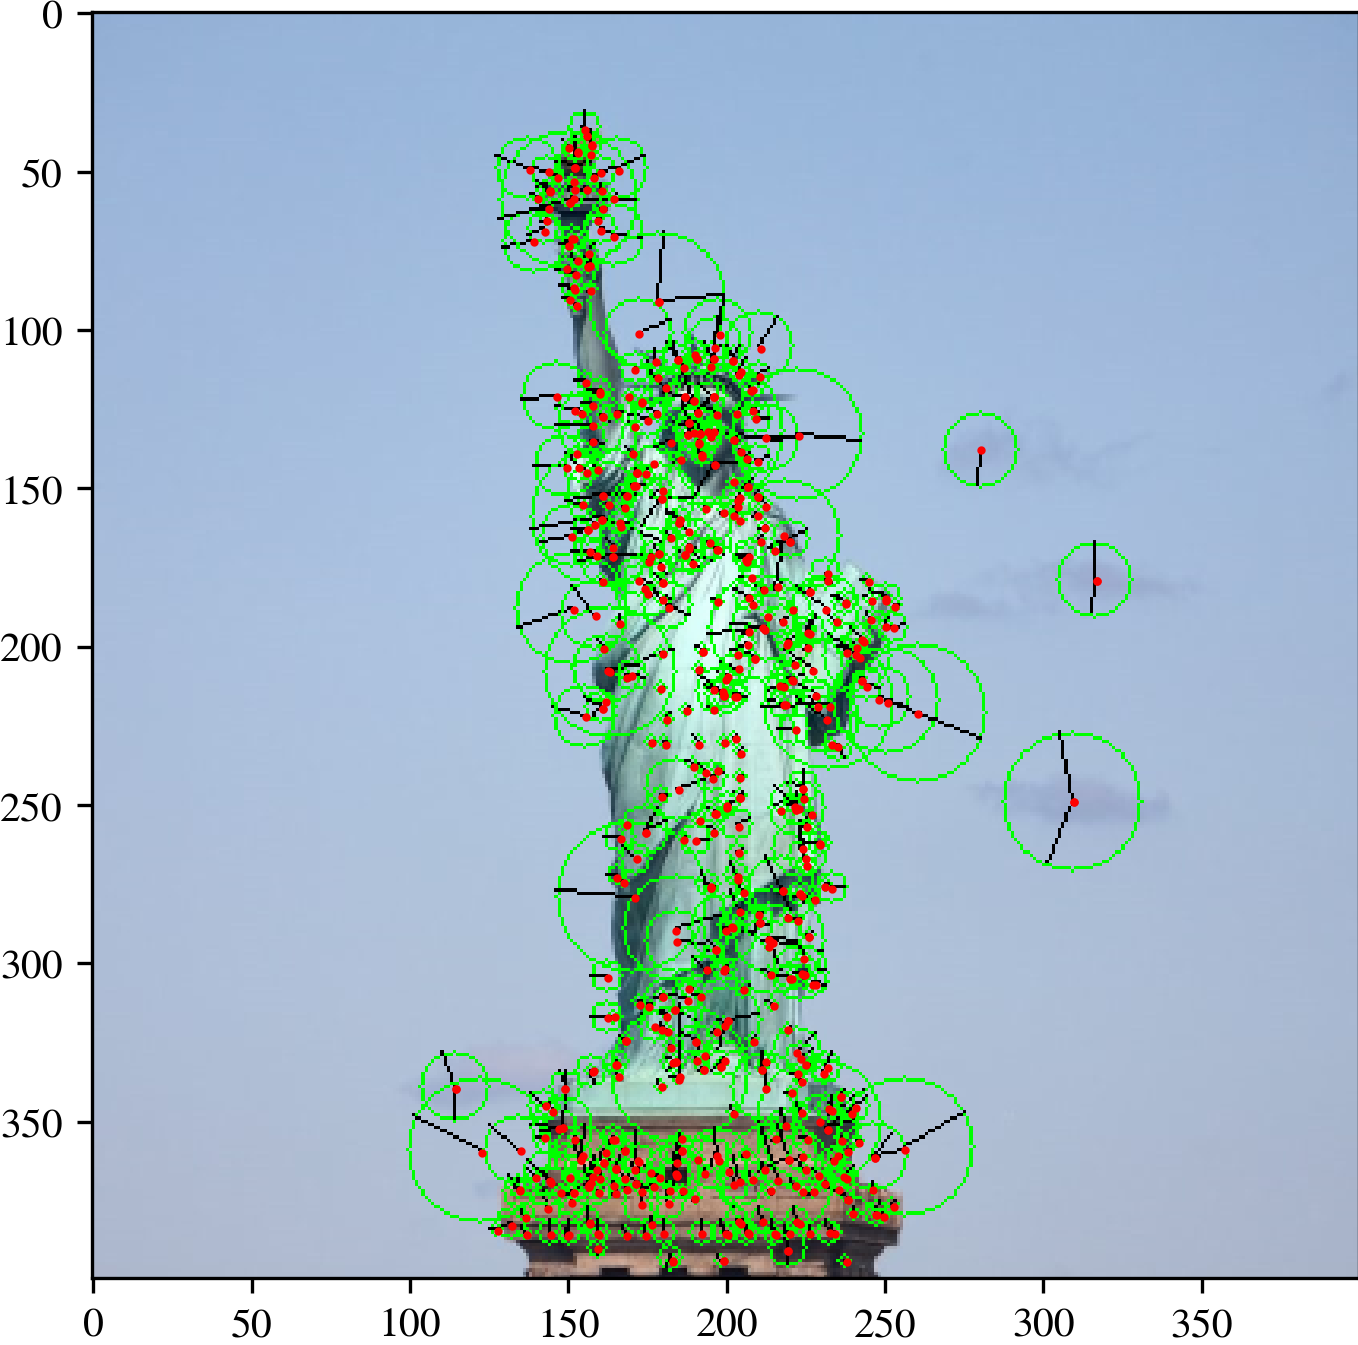
\includegraphics[width=0.5\textwidth]{figs/keypoints_with_descriptors.png}
  \caption{Visualized Keypoints with Descriptors}
\end{figure}

\begin{lstlisting}[language=Python, caption=Comparing with OpenCV]
  sift = cv2.SIFT_create()
  cv_keypoints, cv_descriptors = sift.detectAndCompute(gray_img, None)
  kp = sift.detect(gray_img, None)
  cv_image_with_keypoints = deepcopy(rgb_img)  # Create a copy of the image to draw on

  # Visualize keypoints
  fig, ax = plt.subplots()
  cv_image_with_keypoints = cv2.drawKeypoints(
      cv_image_with_keypoints,
      kp,
      cv_image_with_keypoints,
      flags=cv2.DRAW_MATCHES_FLAGS_DRAW_RICH_KEYPOINTS,
  )
  ax.imshow(cv_image_with_keypoints)
  plt.tight_layout()
  if save:
      plt.savefig(
          "report/figs/opencv_sift.png",
          dpi=300,
          bbox_inches="tight",
          pad_inches=0,
      )
\end{lstlisting}

% 2 subfigures, each with different caption
\begin{figure}[ht!]
  \centering
  \begin{minipage}{0.45\textwidth}
    \centering
    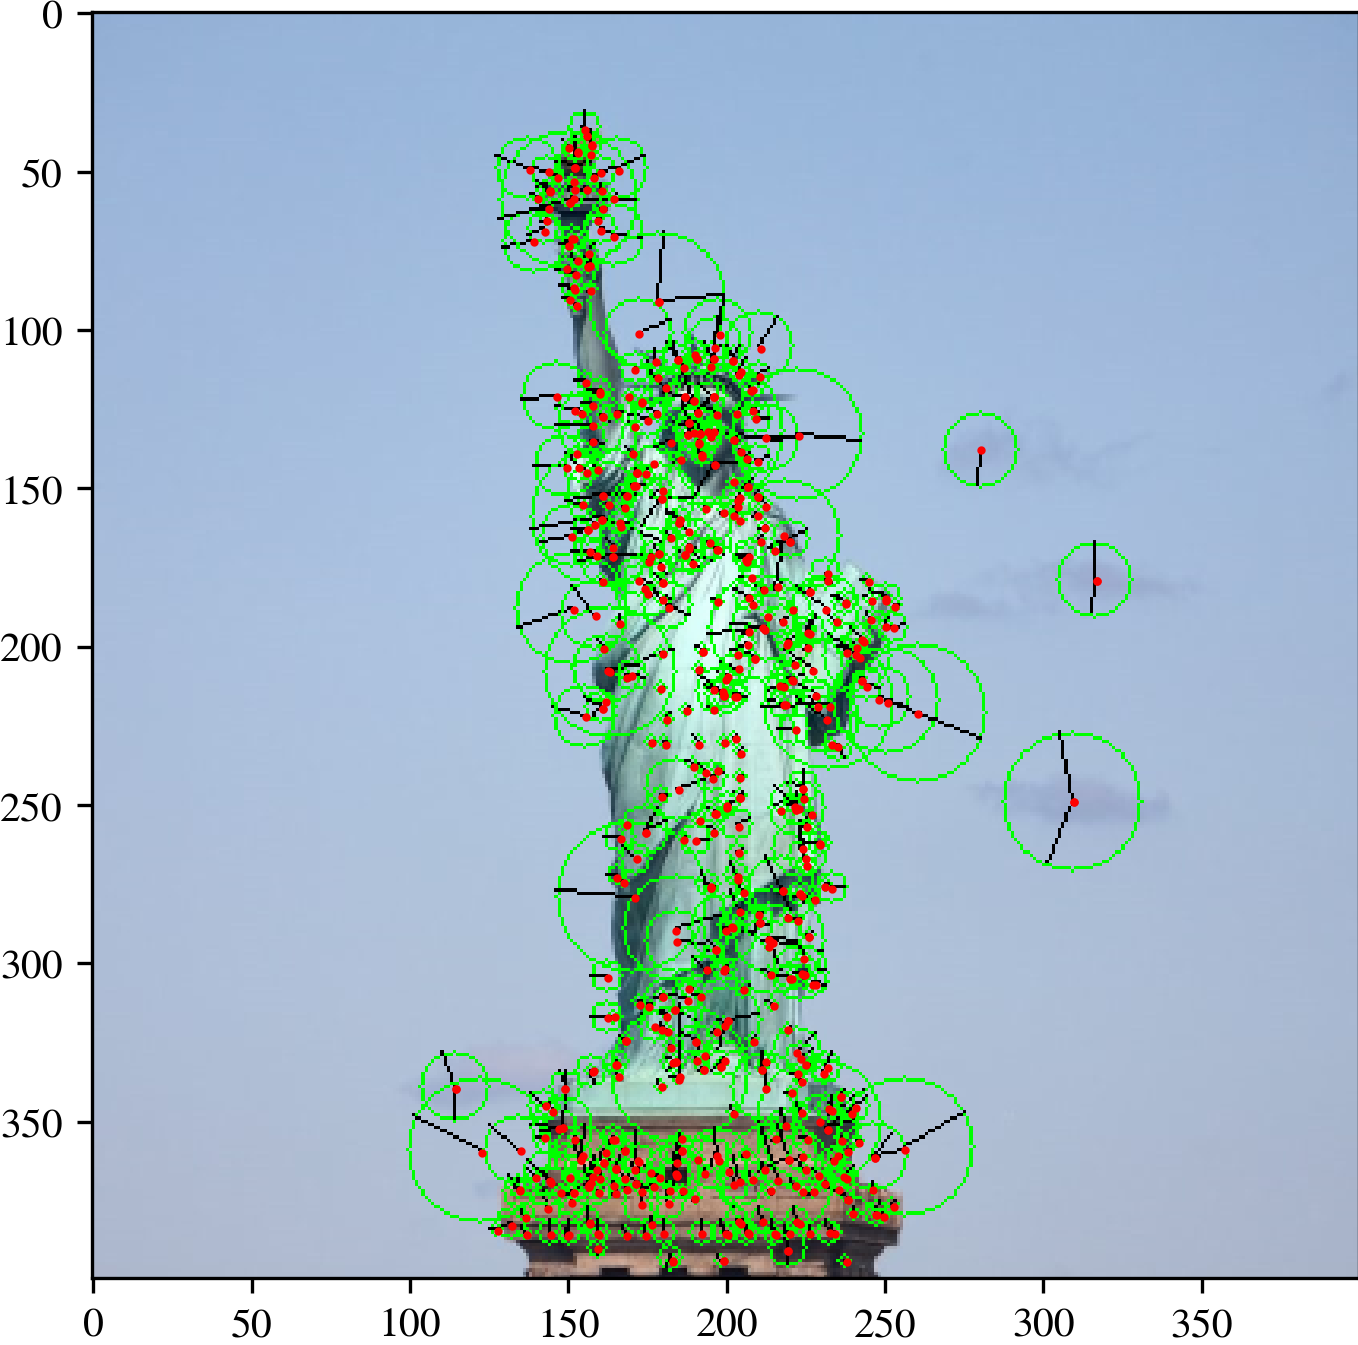
\includegraphics[width=0.9\textwidth]{figs/keypoints_with_descriptors.png} % first figure itself
    \caption{Visualized Keypoints with Descriptors}
  \end{minipage}
  \quad
  \begin{minipage}{0.45\textwidth}
    \centering
    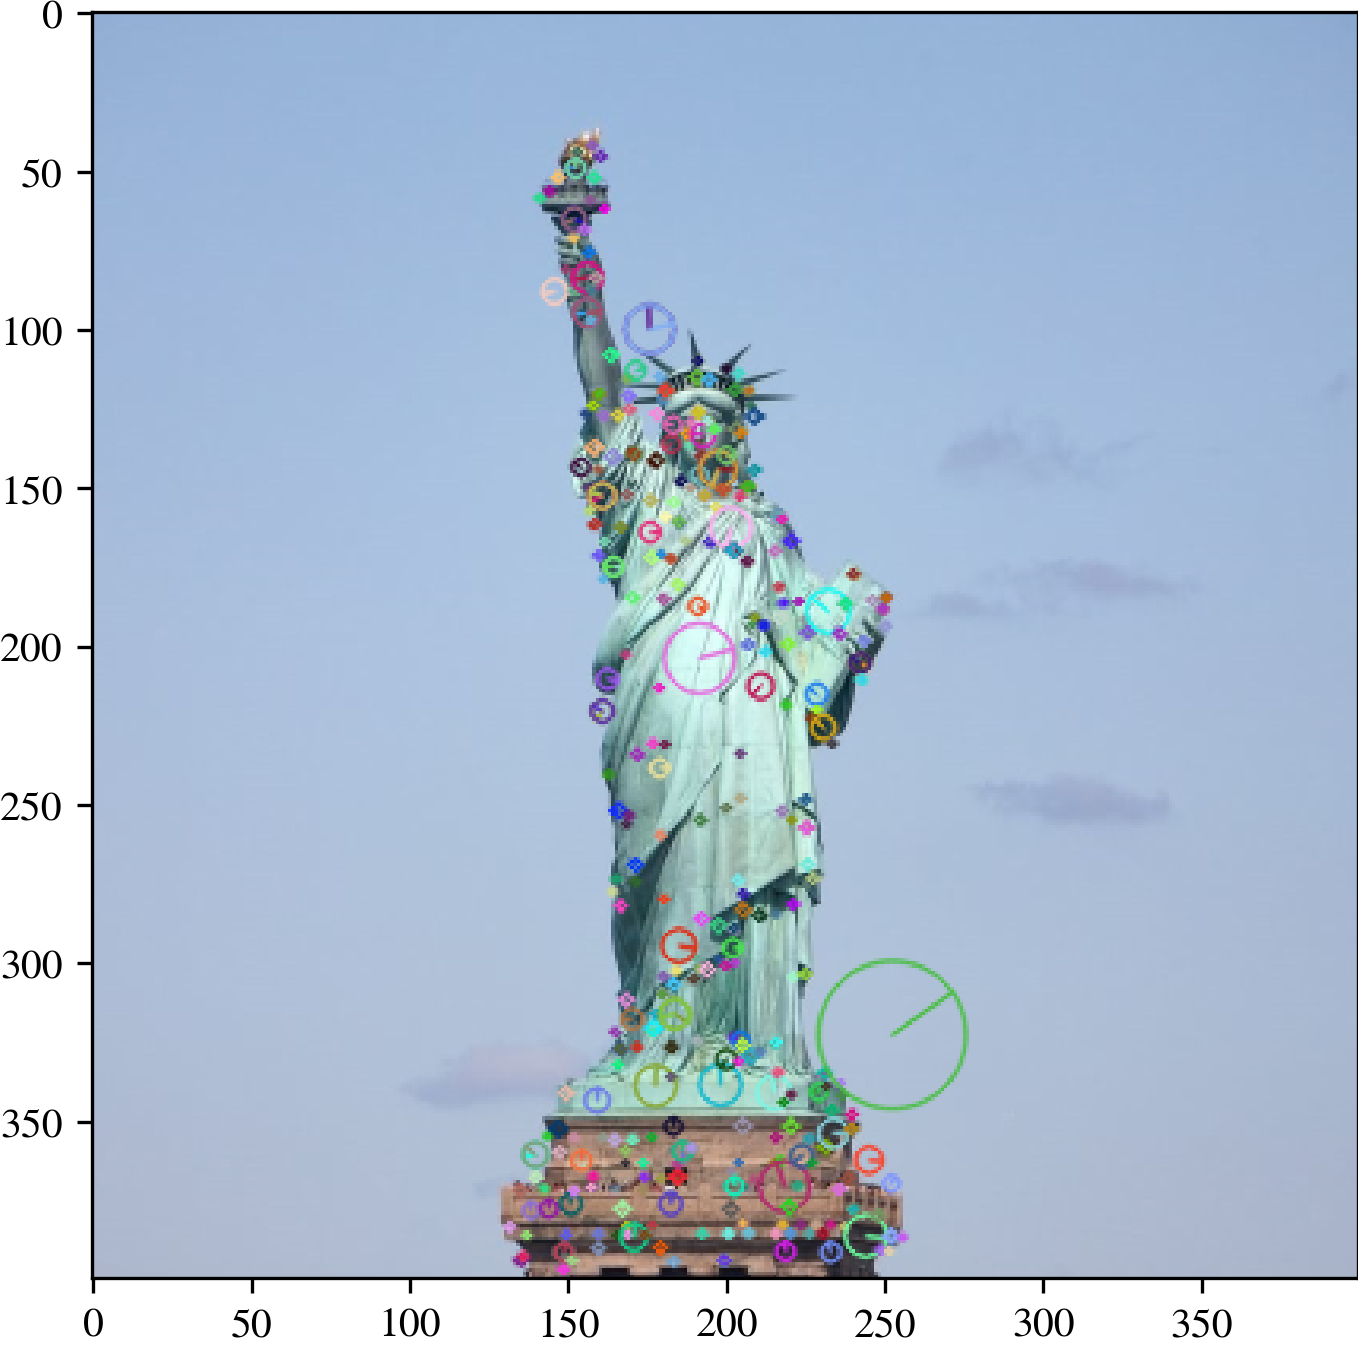
\includegraphics[width=0.9\textwidth]{figs/opencv_sift.png} % second figure itself
    \caption{OpenCV Keypoints}
  \end{minipage}
\end{figure}

\newpage

\begin{lstlisting}[language=Python, caption=Matching keypoints]
  img1_path = "liberty1.png"
  img2_path = "liberty2.png"

  img1_res, cv_img1_res = task1(img1_path, save=True)
  img2_res, cv_img2_res = task1(img2_path, save=False)

  def match(img1_res, img2_res, img1_path, img2_path):
      img1 = cv2.imread(img1_path, 0)
      img2 = cv2.imread(img2_path, 0)
      FLANN_INDEX = 0
      index_params = dict(algorithm=FLANN_INDEX, trees=5)
      search_params = dict(checks=50)

      # Initialize FLANN
      flann = cv2.FlannBasedMatcher(index_params, search_params)
      descriptors1 = np.array(img1_res[1], dtype=np.float32)
      descriptors2 = np.array(img2_res[1], dtype=np.float32)
      matches = flann.knnMatch(descriptors1, descriptors2, k=2)

      # Apply Lowe's ratio test
      valid_matches = []
      for match1, match2 in matches:
          if match1.distance < 0.7 * match2.distance:
              valid_matches.append(match1)

      # Estimate homography
      source_points = np.float32(
          [img1_res[0][m.queryIdx].pt for m in valid_matches]
      ).reshape(-1, 1, 2)
      destination_points = np.float32(
          [img2_res[0][m.trainIdx].pt for m in valid_matches]
      ).reshape(-1, 1, 2)

      homography = cv2.findHomography(
          source_points, destination_points, cv2.RANSAC, 5.0)[0]

      # Draw template in scene image
      height, width = img1.shape
      points = np.float32(
          [[0, 0], [0, height - 1], [width - 1, height - 1], [width - 1, 0]]
      ).reshape(-1, 1, 2)
      transformed_points = cv2.perspectiveTransform(points, homography)

      img2 = cv2.polylines(
          img2, [np.int32(transformed_points)], True, 255, 3, cv2.LINE_AA
      )

      # Create new image to draw matches
      height1, width1 = img1.shape
      height2, width2 = img2.shape
      new_width = width1 + width2
      new_height = max(height1, height2)
      height_diff = int((height2 - height1) / 2)
      combined_img = np.zeros((new_height, new_width, 3), np.uint8)

      for i in range(3):
          combined_img[height_diff : height_diff + height1, :width1, i] = img1
          combined_img[:height2, width1 : width1 + width2, i] = img2

      # Draw matches
      for match in valid_matches:
          point1 = (
              int(img1_res[0][match.queryIdx].pt[0]),
              int(img1_res[0][match.queryIdx].pt[1] + height_diff))
          point2 = (
              int(img2_res[0][match.trainIdx].pt[0] + width1),
              int(img2_res[0][match.trainIdx].pt[1]))
          cv2.line(combined_img, point1, point2, (255, 0, 0))
      return combined_img

  combined_img = match(img1_res, img2_res, img1_path, img2_path)
  cv_combined_img = match(cv_img1_res, cv_img2_res, img1_path, img2_path)

  plt.imshow(combined_img)
  plt.tight_layout()
  plt.savefig("report/figs/matches.png",
               dpi=300, bbox_inches="tight", pad_inches=0)

  plt.imshow(cv_combined_img)
  plt.tight_layout()
  plt.savefig("report/figs/opencv_matches.png",
               dpi=300, bbox_inches="tight", pad_inches=0)
\end{lstlisting}

% 2 subfigures, each with different caption
\begin{figure}[ht!]
  \centering
  \begin{minipage}{0.45\textwidth}
    \centering
    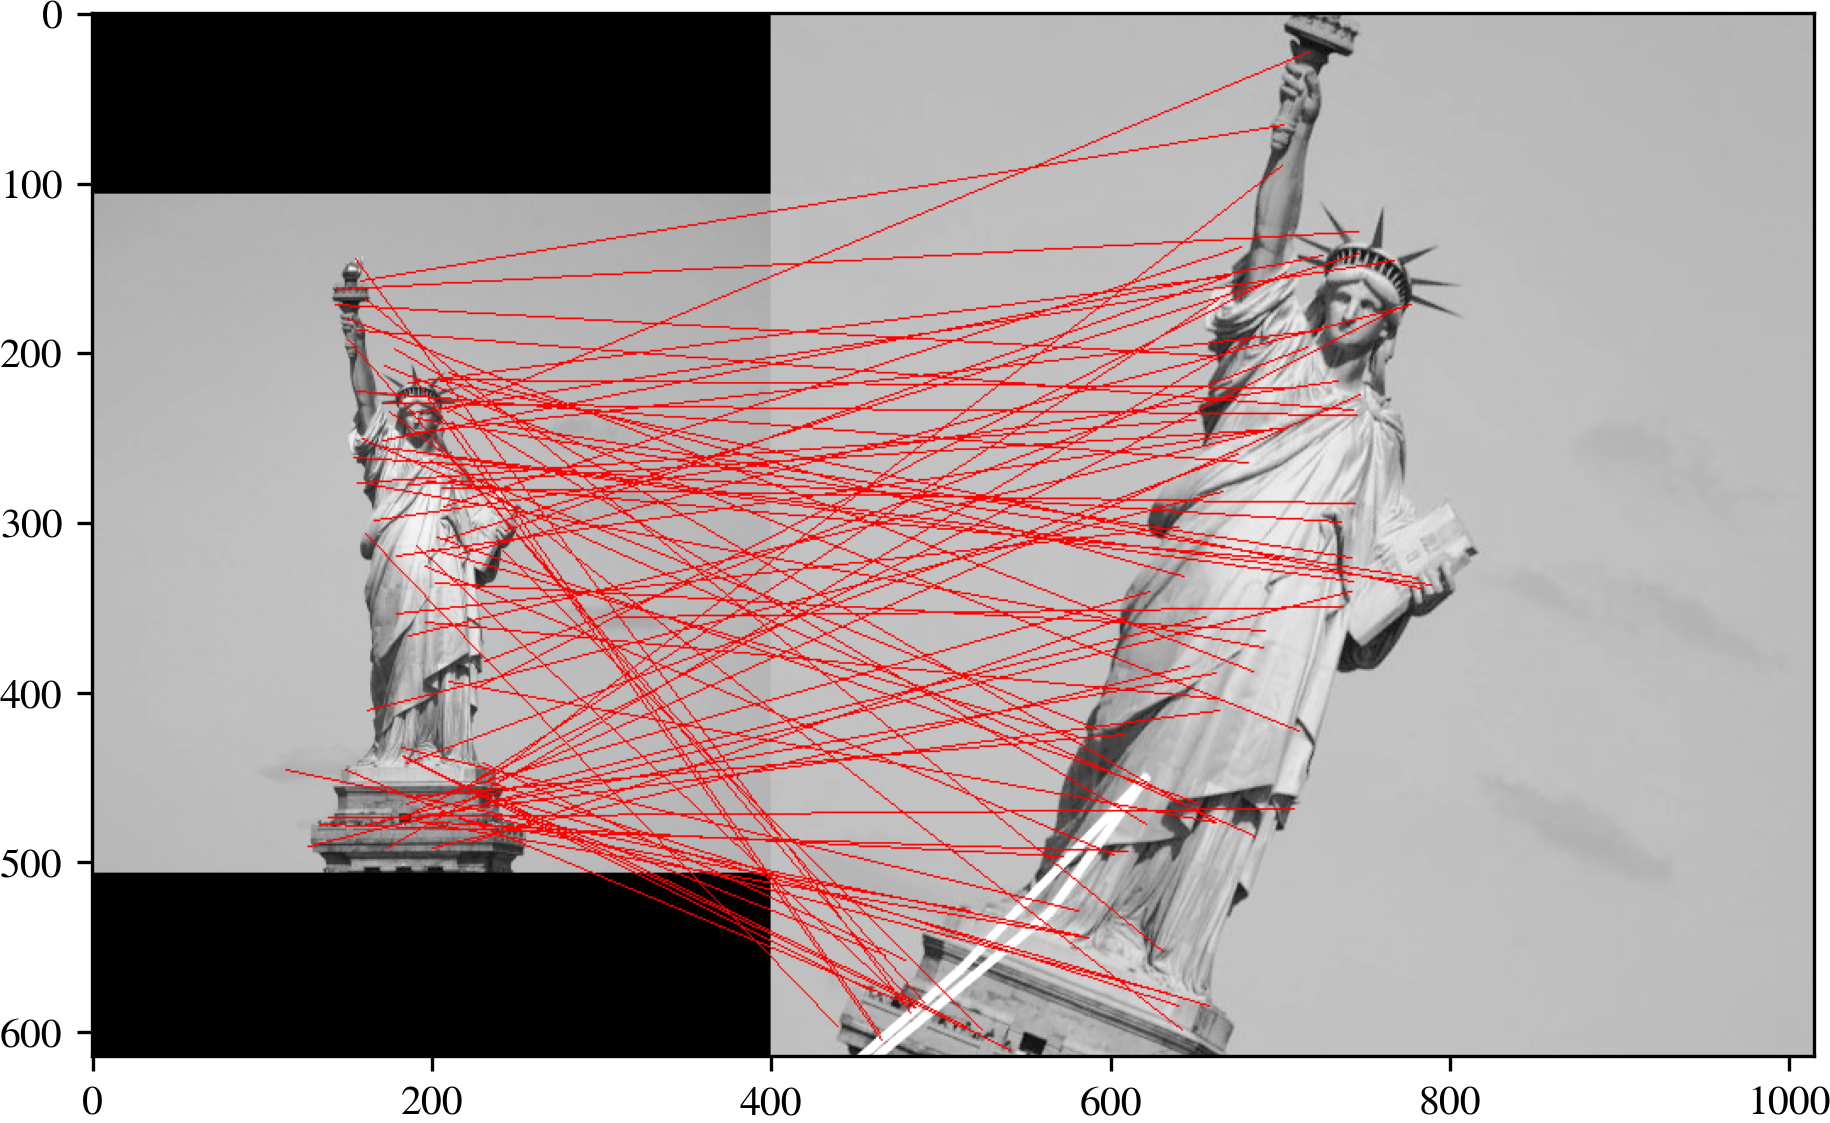
\includegraphics[width=\textwidth]{figs/matches.png} % first figure itself
    \caption{Matches}
  \end{minipage}
  \quad
  \begin{minipage}{0.45\textwidth}
    \centering
    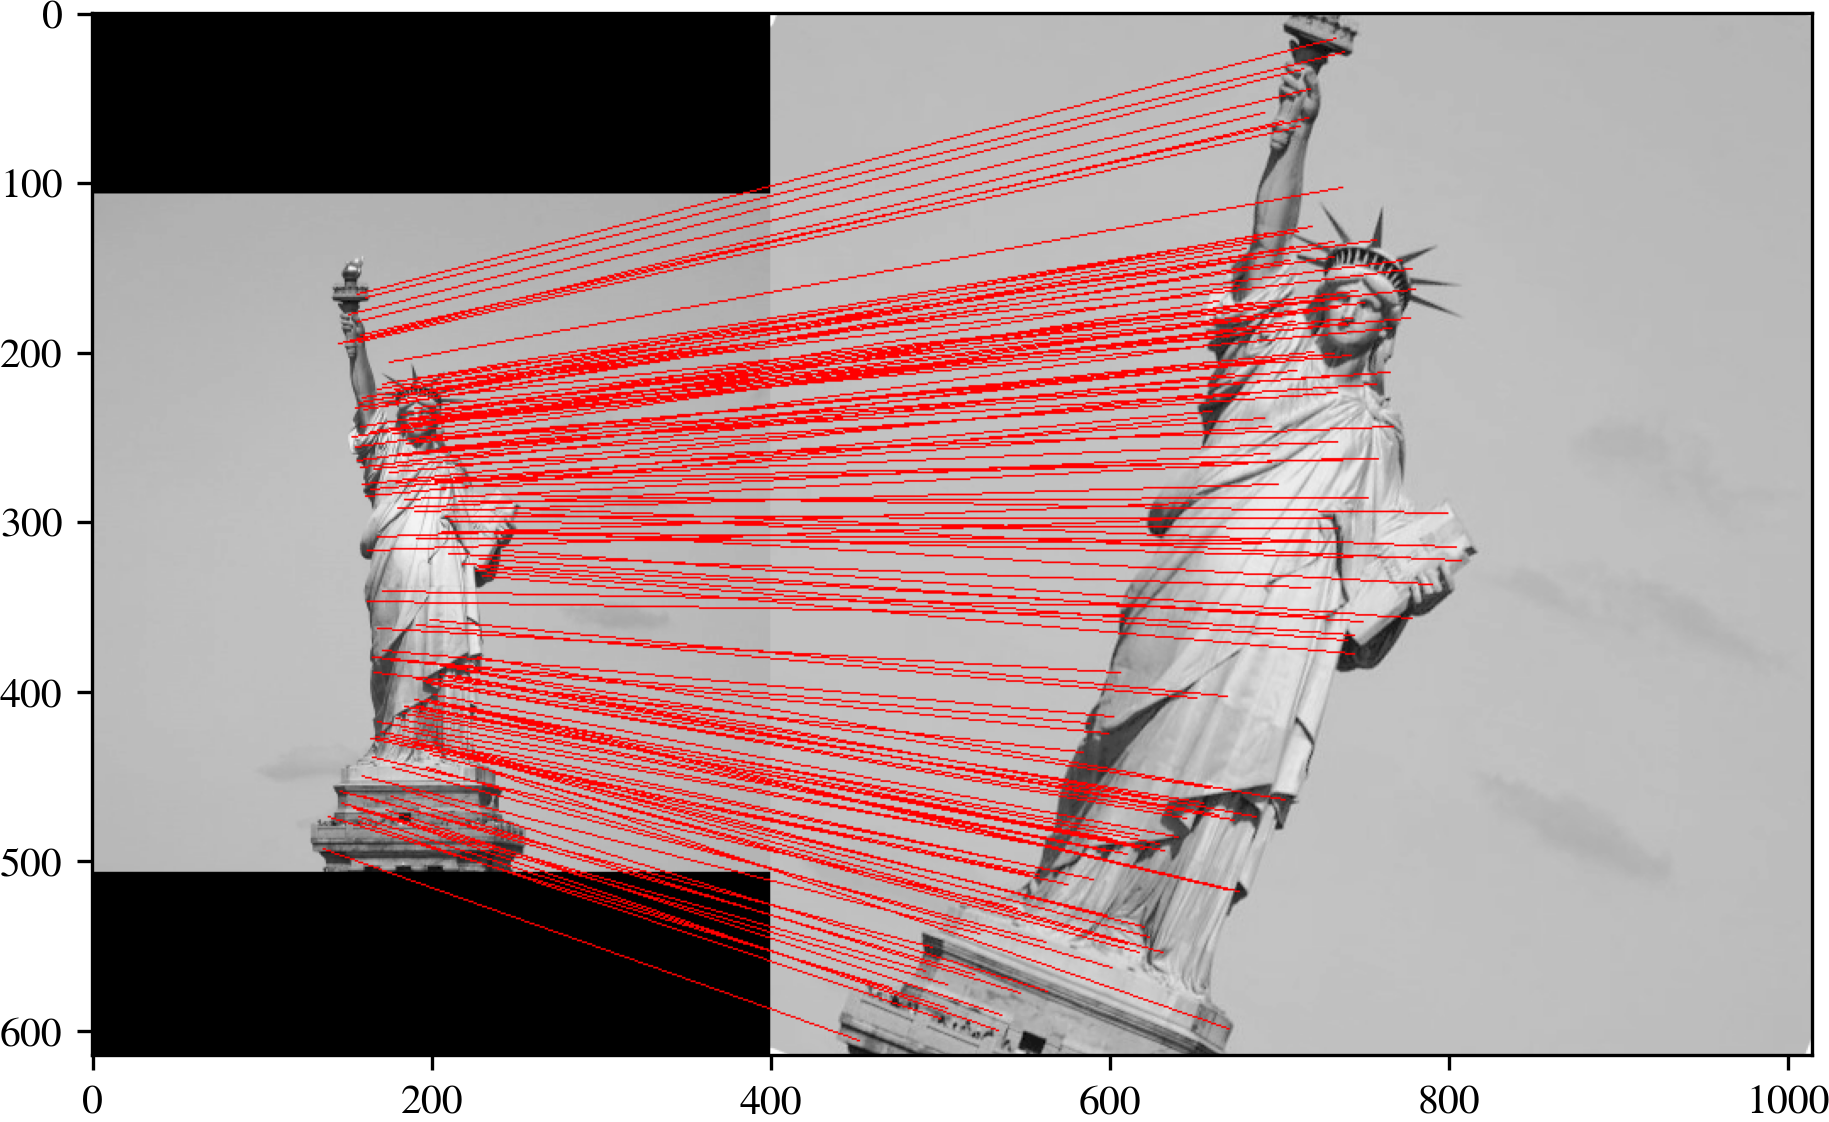
\includegraphics[width=\textwidth]{figs/opencv_matches.png} % second figure itself
    \caption{OpenCV Matches}
  \end{minipage}
\end{figure}

\newpage
\section{Task 2 -- Image Stitching}

Continuing from the previous task, we now stitch the two images together. We begin by loading the images and extracting the keypoints and descriptors using the same method as in the previous task.

\begin{lstlisting}[language=Python, caption=Loading images and applying SIFT]
  # Load the images
  img1_path = "left.png"
  img2_path = "right.png"
  img1 = cv2.imread(img1_path)
  img2 = cv2.imread(img2_path)

  plt.imshow(img1[:, :, ::-1])
  plt.tight_layout()
  plt.savefig("report/figs/left.png",
               dpi=300, bbox_inches="tight", pad_inches=0)
  
  plt.imshow(img2[:, :, ::-1])
  plt.tight_layout()
  plt.savefig("report/figs/right.png",
               dpi=300, bbox_inches="tight", pad_inches=0)

  # Perform task1 on both images
  img1_res, cv_img1_res = task1(img1_path, save=False)
  img2_res, cv_img2_res = task1(img2_path, save=False)

  # Extract keypoints and descriptors
  kp1 = img1_res[0]
  kp2 = img2_res[0]
  descriptors1 = np.array(img1_res[1], dtype=np.float32)
  descriptors2 = np.array(img2_res[1], dtype=np.float32)
\end{lstlisting} 

% 2 subfigures, each with different caption
\begin{figure}[ht!]
  \centering
  \begin{minipage}{0.45\textwidth}
    \centering
    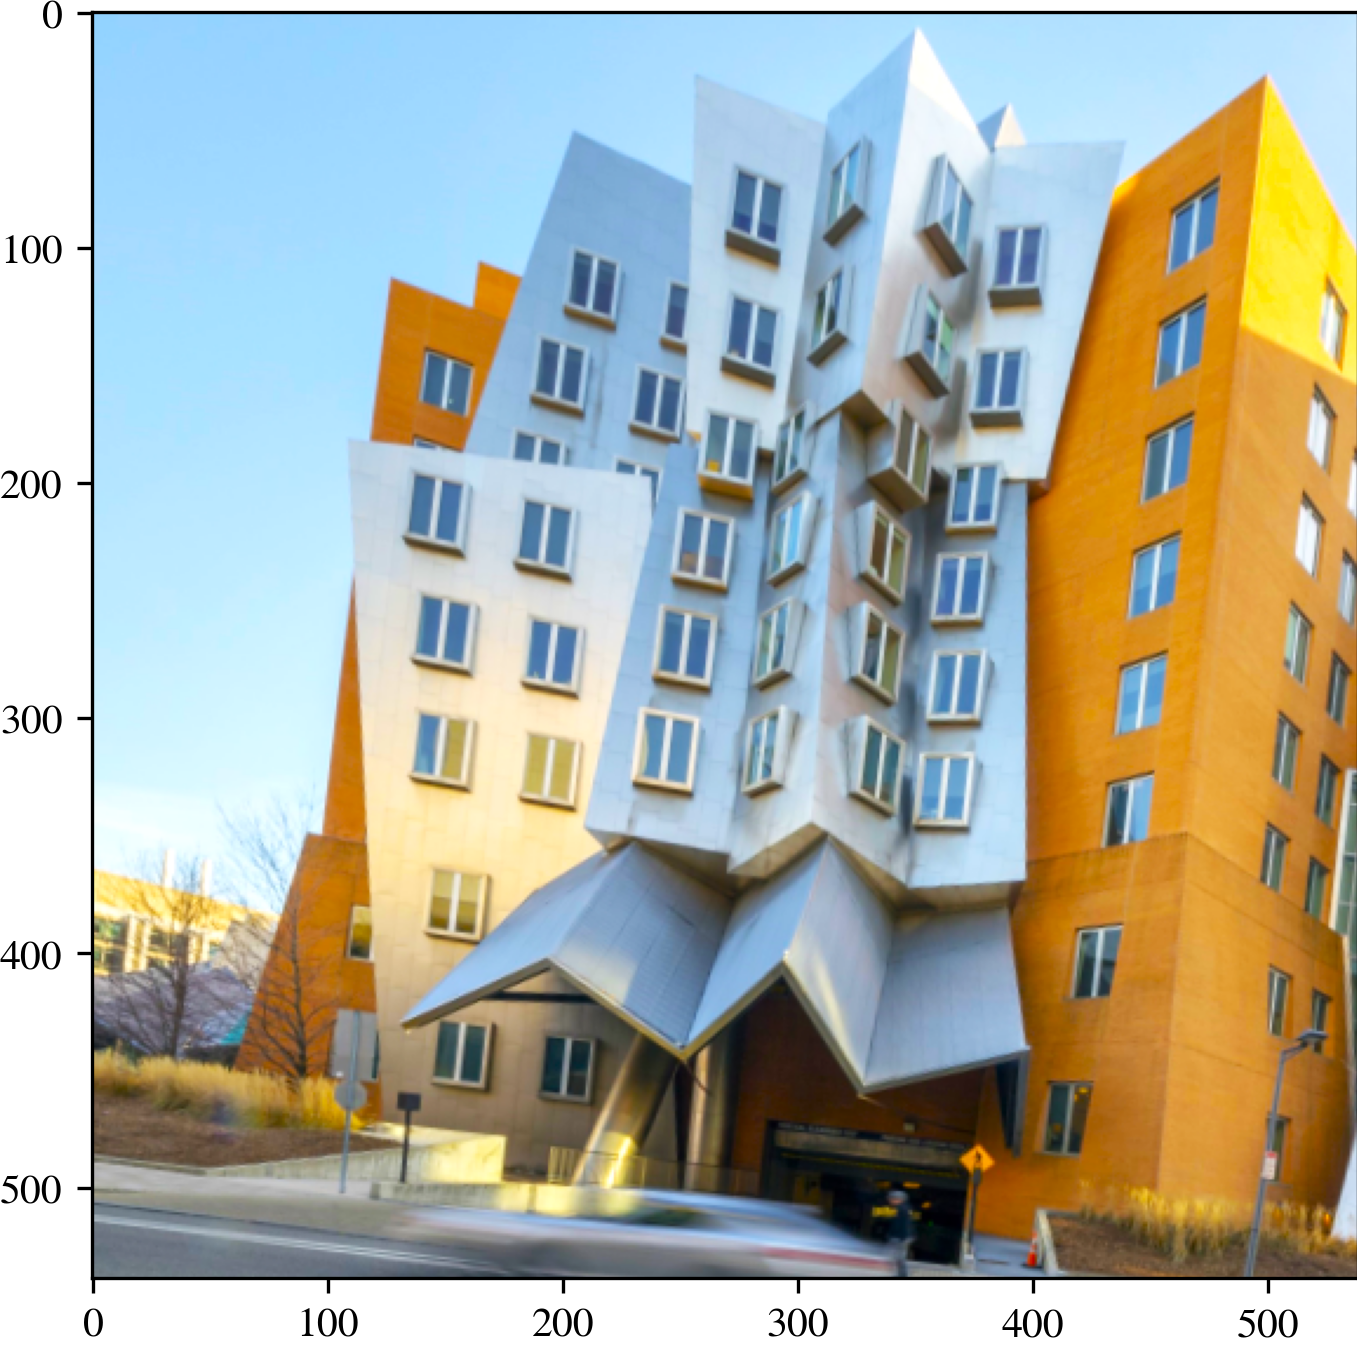
\includegraphics[width=0.9\textwidth]{figs/left.png} % first figure itself
    \caption{Left Image}
  \end{minipage}
  \quad
  \begin{minipage}{0.45\textwidth}
    \centering
    
\includegraphics[width=0.9\textwidth]{figs/right.png} % second figure itself
    \caption{Right Image}
  \end{minipage}
\end{figure}

Next, we proceed to match the keypoints and stitch the images together.

\begin{lstlisting}[language=Python, caption=Matching keypoints and stitching images]
  # Set parameters for matching
  ratio = 0.85
  min_match = 10
  smoothing_window_size = 500

  # Perform matching
  matcher = cv2.BFMatcher()
  raw_matches = matcher.knnMatch(descriptors1, descriptors2, k=2)

  # Filter matches
  good_points = []
  good_matches = []
  for m1, m2 in raw_matches:
      if m1.distance < ratio * m2.distance:
          good_points.append((m1.trainIdx, m1.queryIdx))
          good_matches.append([m1])

  # Find homography if enough matches
  if len(good_points) > min_match:
      image1_kp = np.float32([kp1[i].pt for (_, i) in good_points])
      image2_kp = np.float32([kp2[i].pt for (i, _) in good_points])
      H, status = cv2.findHomography(image2_kp, image1_kp, cv2.RANSAC, 5.0)

  # Function to create a mask for blending
  def create_mask(img1, img2, version):
      # Calculate dimensions
      height_img1 = img1.shape[0]
      width_img1 = img1.shape[1]
      width_img2 = img2.shape[1]
      height_panorama = height_img1
      width_panorama = width_img1 + width_img2
      offset = int(smoothing_window_size / 2)
      barrier = img1.shape[1] - int(smoothing_window_size / 2)
      mask = np.zeros((height_panorama, width_panorama))
      # Create mask
      if version == "left_image":
          mask[:, barrier - offset : barrier + offset] = np.tile(
              np.linspace(1, 0, 2 * offset).T, (height_panorama, 1))
          mask[:, : barrier - offset] = 1
      else:
          mask[:, barrier - offset : barrier + offset] = np.tile(
              np.linspace(0, 1, 2 * offset).T, (height_panorama, 1))
          mask[:, barrier + offset :] = 1
      return cv2.merge([mask, mask, mask])

  # Calculate dimensions for panorama
  height_img1 = img1.shape[0]
  width_img1 = img1.shape[1]
  width_img2 = img2.shape[1]
  height_panorama = height_img1
  width_panorama = width_img1 + width_img2

  # Create panorama with left image
  panorama1 = np.zeros((height_panorama, width_panorama, 3))
  mask1 = create_mask(img1, img2, version="left_image")
  panorama1[0 : img1.shape[0], 0 : img1.shape[1], :] = img1
  panorama1 *= mask1

  # Create panorama with right image
  mask2 = create_mask(img1, img2, version="right_image")
  panorama2 = cv2.warpPerspective(img2, H, (width_panorama, height_panorama)) * mask2
  result = panorama1 + panorama2

  # Crop the result
  rows, cols = np.where(result[:, :, 0] != 0)
  min_row, max_row = min(rows), max(rows) + 1
  min_col, max_col = min(cols), max(cols) + 1
  final_result = result[min_row:max_row, min_col:max_col, :]
  panorama = np.clip(final_result, 0, 255).astype(np.uint8)

  # Display and save the result
  plt.imshow(panorama[:, :, ::-1])
  plt.title("Stitched Image")
  plt.tight_layout()
  plt.savefig("report/figs/stitched.png",
               dpi=300, bbox_inches="tight", pad_inches=0)
\end{lstlisting}

\begin{figure}[H]
    \centering
    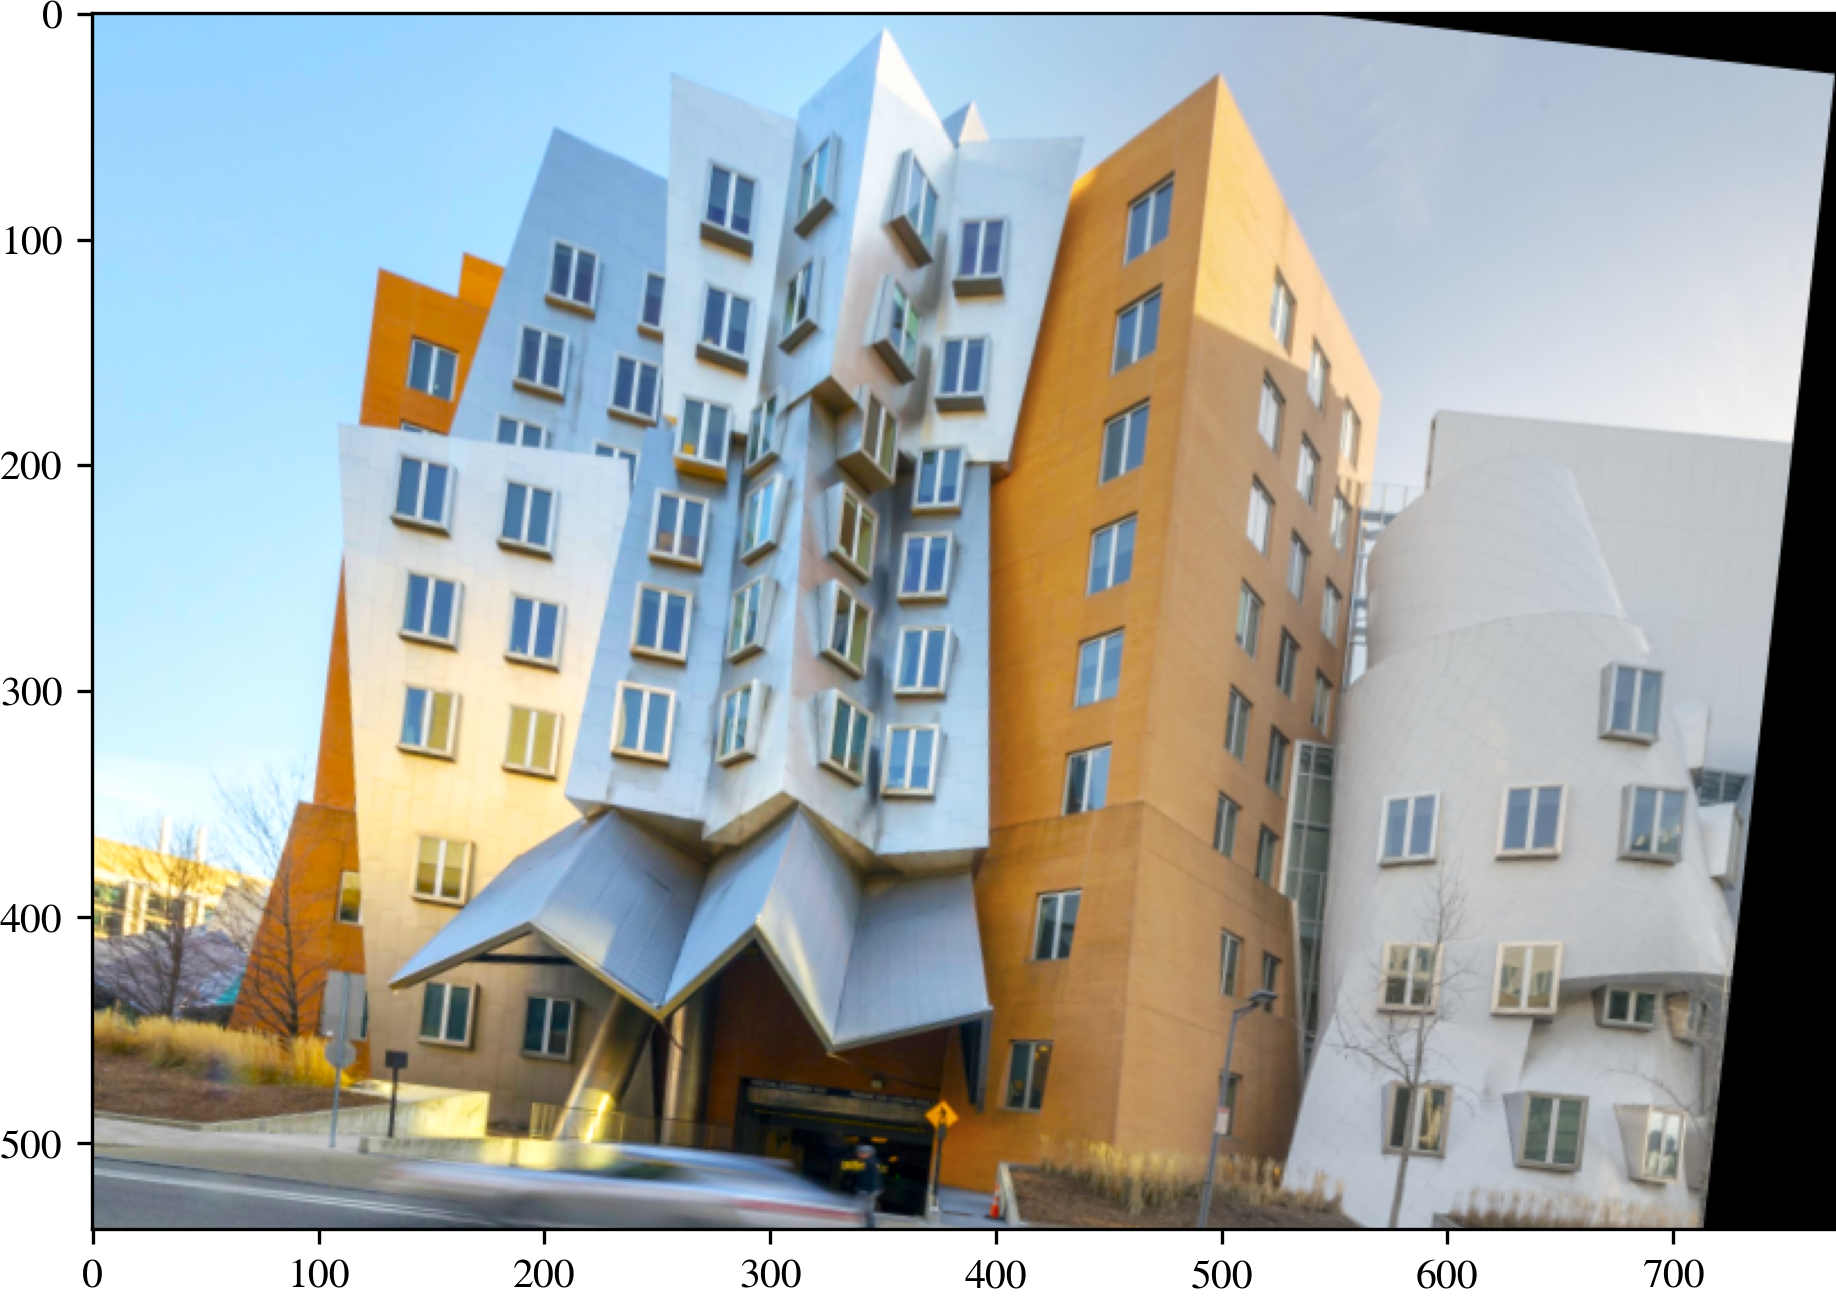
\includegraphics[width=0.65\textwidth]{figs/stitched.png}
    \caption{Stitched Image}
  \end{figure}

\end{document}